\documentclass[final]{qutthesis}

% The document class file
% *************************************
% ENN595-1 Assessment 2B: Project Progress Written Report
% *************************************
% Investigation of Primitive-Space Scene Change Detection in Underwater 3D Gaussian Splatting Models
% Author: Joshua Hecke (n11585382)
% Supervisors: Prof. Niko Sünderhauf & Dr. Scarlett Raine (QUT Centre for Robotics)

% ***************************************************
% LaTeX Packages
% ***************************************************

\usepackage{cite}				 %Allows abbreviated numerical citations.
\usepackage{pdfpages}			 %Allows you to include full-page pdfs.
\usepackage{wrapfig}			 %Lets you wrap text around figures.
\usepackage{bm} 				 %Bolded maths characters.
\usepackage{upgreek}			 %Upright Greek characters.
\usepackage{dsfont}				 %Double-struck fonts.
\usepackage{simplewick}			 %For typesetting Wick contractions.
\usepackage{mathtools}		     %Can be used to fine-tune the maths presentation.	
\usepackage{framed}			     %For boxed text.
\usepackage{microtype}			 %pdfLaTeX will fix your kerning.
\usepackage{marvosym}			 %Include symbols (like the Euro symbol, etc.).
\usepackage{color}				 %Nice for scalable pdf graphics using InkScape.
\usepackage{transparent}	     %Nice for scalable pdf graphics using InkScape.
\usepackage{placeins}			 %Lets you put in a \FloatBarrier to stop figures floating past this command.
\usepackage{mdframed,mdwlist}    %Use these for nice lists (less white space).
\usepackage{setspace}
\usepackage{graphicx}            %Enhanced support for graphics.
\usepackage{float}               %Improved interface for floating objects. 
\usepackage{longtable}           %Allow tables to flow over page boundaries.
\usepackage{mathdots}            %Changed the basic LaTeX and plain TeX commands.
\usepackage{eucal}               %Font shape definitions to use the Euler script symbols in math mode.
\usepackage{array}               %Extending the array and tabular environments.
\usepackage{stmaryrd}            %The StMary’s Road symbol font.
\usepackage{amsthm}              %St Mary Road symbols for theoretical computer science. 
\usepackage{pifont}              %Access to PostScript standard Symbol and Dingbats fonts.
\usepackage{lipsum}              %Easy access to the Lorem Ipsum dummy text.
\usepackage{enumerate}           %Enumerate with redefinable labels. 
\usepackage[all]{xy}             %This is a special package for drawing diagrams.
\usepackage{amsmath}             %ATypesetting theorems (AMS style).
\usepackage{amssymb}             %Provided an extended symbol collection.
\usepackage[utf8]{inputenc}      %Allowed all displayable utf8 characters to be available as input.
\usepackage{fancyhdr}            %Extensive control of page headers and footers.
\usepackage{blindtext}           %Produced 'blind' text for testing.
\usepackage{tikz}                %To create graphic elements.
\usepackage[figuresright]{rotating}	%Allows large tables to be rotated to landscape.
\usepackage{multirow}
\usepackage{multicol}
\usetikzlibrary{shapes.geometric, arrows}
%You can add more packages here if you need
\usepackage{siunitx}
\usepackage{xltabular}
\usepackage{pgfgantt}
\usepackage{paralist} % remove line space in the enumeration environment
\usepackage{parskip}
\usepackage{subcaption}
\usepackage{array,blindtext, booktabs,tabularx}
%\usepackage{showframe}
\usepackage{pdfpages}
%insert pdf files 
\usepackage{soul}
%fix underline issues
\usepackage[acronym,nopostdot,style=long3col,toc, nonumberlist]{glossaries}
%grossaries
\usepackage{array}
\newcolumntype{x}[1]{>{\centering\arraybackslash\hspace{0pt}}p{#1}}
\newcolumntype{P}[1]{>{\centering\arraybackslash}p{#1}}
%column centering and width
% % % % % % % % % % % % % % %
\usepackage{algorithm}      %
\usepackage{algpseudocode}  %
% % % % % % % % % % % % % % %

%This defines some macros that implement Latin abbreviations
%COMMENT OUT OR DELETE IF UNDESIRED.
\newcommand{\via}{\textit{via}} %Italicised via.
\newcommand{\ie}{\textit{i.e.}} %Literally.
\newcommand{\eg}{\textit{e.g.}} %For example.
\newcommand{\etc}{\textit{etc.}} %So on...
\newcommand{\vv}{\textit{vice versa}} %And the other way around.
\newcommand{\viz}{\textit{viz}.} %Resulting in.
\newcommand{\cf}{\textit{cf}.} %See, or 'consistent with'.
\newcommand{\apr}{\textit{a priori}} %Before the fact.
\newcommand{\apo}{\textit{a posteriori}} %After the fact.
\newcommand{\vivo}{\textit{in vivo}} %In the flesh.
\newcommand{\situ}{\textit{in situ}} %On location.
\newcommand{\silico}{\textit{in silico}} %Simulation.
\newcommand{\vitro}{\textit{in vitro}} %In glass.
\newcommand{\vs}{\textit{versus}} %James \vs{} Pete.
\newcommand{\ala}{\textit{\`{a} la}} %In the manner of...
\newcommand{\apriori}{\textit{a priori}} %Before hand.
\newcommand{\etal}{\textit{et al.}} %And others, with correct punctuation.
\newcommand{\naive}{na\"\i{}ve} %Queen Amidala is young and \naive{}.



% ***************************************************
% Title page Metadata
% ***************************************************

\title{Investigation of Primitive-Space Scene Change Detection in Underwater 3D Gaussian Splatting Models}
\author{Joshua Hecke}
\currentdegrees{Bachelor of Engineering (Honours) / Master of Robotics and Artificial Intelligence\\(Student ID: n11585382)}
\date{October 2026}
\submittedfor{Bachelor of Engineering (Honours) / Master of Robotics and Artificial Intelligence}

\school{School of Electrical Engineering and Robotics}
\faculty{Faculty of Engineering}
\university{Queensland University of Technology}
\supervisor{Principal Supervisor: Prof. Niko S{\"u}nderhauf}
\asscsupervisor{Associate Supervisor / Domain Contact: Dr. Scarlett Raine}

% --- Acronyms / Glossaries ---
\makeglossaries
\newacronym{3dgs}{3DGS}{3D Gaussian Splatting}
\newacronym{scd}{SCD}{Scene Change Detection}
\newacronym{oscd}{O-SCD}{Online Scene Change Detection}
\newacronym{psnr}{PSNR}{Peak Signal-to-Noise Ratio}
\newacronym{ssim}{SSIM}{Structural Similarity Index Measure}
\newacronym{lpips}{LPIPS}{Learned Perceptual Image Patch Similarity}
\newacronym{sfm}{SfM}{Structure from Motion}
\newacronym{aims}{AIMS}{Australian Institute of Marine Science}
\newacronym{ecorrap}{EcoRRAP}{Reef Restoration and Adaptation Program}
\newacronym{qcr}{QCR}{QUT Centre for Robotics}
\newacronym{hpc}{HPC}{High-Performance Computing}
\newacronym{sugar}{SuGaR}{Surface-Aligned Gaussian Splatting}
\newacronym{dtn}{DTN}{Data Transfer Node}
\newacronym{sdf}{SDF}{Signed Distance Function}
\newacronym{nerf}{NeRF}{Neural Radiance Fields}
\newacronym{vram}{VRAM}{Video Random Access Memory}
\newacronym{auv}{AUV}{Autonomous Underwater Vehicle}

% *************************************************
% Front Matter
% *************************************************
\begin{document}

\frontmatter 
\pagestyle{myfancy}

% Assemble title page
\maketitle

%--------------------------------------
\chapter{Keywords}
\normalfont
% ***************************************************
% Keywords
% ***************************************************

\noindent
\textbf{Primary Research Keywords:}
\begin{itemize}
    \item 3D Gaussian Splatting (3DGS)
    \item Underwater 3D Reconstruction and Optical Medium Restoration
    \item Primitive-Space Scene Change Detection (SCD)
    \item Online Scene Change Detection (O-SCD)
    \item Surface-Aligned Gaussian Regularization (SuGaR)
    \item Signed Distance Functions (SDF) and Watertight Poisson Surface Meshing
    \item Wavelength-Dependent Light Attenuation and Aquatic Backscatter Inversion
    \item Marine Photogrammetry and Autonomous Underwater Vehicle (AUV) Surveys
    \item High-Resolution Benthic Coral Reef Structural and Rugosity Monitoring
    \item Reef Restoration and Adaptation Program (EcoRRAP)
    \item High-Performance Computing (HPC) Automated Batch Workflow Architecture
\end{itemize}

\vspace{1.5em}
\noindent
\textbf{Australian and New Zealand Standard Research Classifications (ANZSRC 2020):}
\begin{itemize}
    \item \textbf{460303} -- Computer Vision
    \item \textbf{460309} -- Spatial and Volumetric Information Systems
    \item \textbf{400701} -- Autonomous Systems and Robotics
    \item \textbf{410402} -- Marine and Estuarine Ecology
\end{itemize}

\clearpage

%--------------------------------------
\chapter{Executive Summary}
\normalfont
% ***************************************************
% Executive Summary / Abstract
% ***************************************************

Marine ecosystems, particularly coral reefs, are undergoing unprecedented rates of degradation due to climate-driven thermal stress, bleaching events, and anthropogenic disturbances. Effective ecological conservation and reef restoration necessitate high-frequency, millimetre-accurate three-dimensional structural monitoring. However, traditional marine surveys depend heavily on diver-operated, two-dimensional planar transects and localized quadrats that fail to capture complex volumetric changes, structural breakage, and coral colony growth over time. 

This research project investigates the feasibility and efficacy of primitive-space Scene Change Detection (\gls{scd}) integrated with underwater-optimised 3D Gaussian Splatting (\gls{3dgs}) architectures. Unlike conventional render-then-compare paradigms that suffer from viewpoint dependencies and require pixel-space differencing, direct primitive-space change detection (\gls{oscd}) analyses structural transformations directly within native Gaussian attributes (position, anisotropic covariance, and colour harmonics).

To date, the project has achieved a major preliminary computational milestone: \textbf{15 out of 15 (100\%) full-lifecycle benchmark executions} have succeeded across an automated 6-stage pipeline on the QUT Aqua High-Performance Computing (\gls{hpc}) cluster. Across eight distinct state-of-the-art models evaluated on two real-world underwater shipwreck benchmarks (\textit{Submerged3D} Kwajalein and Tokai Maru) and a dual-state change detection dataset, the pipeline has extracted photorealistic 3D Gaussian representations, watertight surface meshes via Surface-Aligned Gaussian Splatting (\gls{sugar}), and high-fidelity novel view syntheses. Quantitative benchmarking confirms high reconstruction accuracy, with the primitive-space \gls{oscd} engine achieving a Peak Signal-to-Noise Ratio (\gls{psnr}) of $27.08\text{ dB}$, a Structural Similarity Index (\gls{ssim}) of $0.8315$, and a perceptual loss (\gls{lpips}) of $0.3440$.

Importantly, these preliminary executions serve as an essential proof-of-concept benchmark to rigorously evaluate candidate models. The ultimate objective of this thesis requires sensitive, high-density temporal photogrammetry from the \textbf{Australian Institute of Marine Science (\gls{aims}) EcoRRAP project} (a massive 1.35~TB dataset). This dataset is currently undergoing secure inter-institutional data transfer, subject to legal and data-sharing agreements. Building upon the empirical benchmarks established herein, Phase~2 and Phase~3 of the project will transplant the top-performing underwater 3DGS architectures (specifically \textit{3D-UIR} and \textit{SeaSplat}) into the \gls{oscd} pipeline, replacing naive terrestrial splatting backbones. These integrated models will undergo extended cluster optimization on Aqua to eliminate false-positive water column floaters and execute millimetre-precision primitive-space volumetric change tracking for marine conservation.
\vspace{1.5em}
\noindent\textbf{Keywords:} 3D Gaussian Splatting (3DGS), Underwater 3D Reconstruction, Primitive-Space Scene Change Detection, Surface-Aligned Regularization (SuGaR), Optical Attenuation, Marine Photogrammetry, Coral Reef Monitoring, EcoRRAP, High-Performance Computing (HPC).
\clearpage

\tableofcontents
\clearpage
\begingroup
\let\clearpage\relax
\listoftables
\vspace{2em}
\listoffigures
\endgroup
\clearpage

% ***************************************************
\chapter{Statement of Original Authorship}
% ***************************************************
% Statement of Original Authorship
% ***************************************************

The work contained in this progress report has not been previously submitted to meet requirements for an award at this or any other higher education institution. To the best of my knowledge and belief, the report contains no material previously published or written by another person except where due reference is made in the text.

\vspace{3cm}

\noindent
\begin{tabular}{ll}
\textbf{Student Signature:} & Joshua Hecke \\
\addlinespace
\textbf{Student ID:}        & n11585382 \\
\addlinespace
\textbf{Date:}              & \today \\
\end{tabular}
\clearpage

% ***************************************************
\chapter{Acknowledgements}
% ***************************************************
% Acknowledgements
% ***************************************************

I would like to express my sincere gratitude and appreciation to my principal project supervisor, \textbf{Prof. Niko S{\"u}nderhauf}, for his invaluable technical guidance, insightful feedback, and continuous encouragement throughout the conception and computational execution of this research. His expertise in robotics, vision, and deep spatial representations has been instrumental in shaping the theoretical rigour of this project.

I am equally grateful to \textbf{Dr. Scarlett Raine} for her outstanding support as domain contact and research advisor. Her deep domain expertise in underwater computer vision and marine photogrammetry, combined with her proactive coordination of dataset access, has been pivotal in aligning this research with genuine marine science applications.

Special thanks are extended to the \textbf{QUT Centre for Robotics (QCR)} and the \textbf{Australian Institute of Marine Science (AIMS)} for their institutional support and partnership in the EcoRRAP monitoring project. I also acknowledge the high-performance computing resources and technical support provided by the \textbf{QUT High Performance Computing (HPC) Support Team}, particularly regarding the Aqua cluster infrastructure.

Finally, I would like to thank my peers, faculty members, and family for their unwavering support throughout the Honours and Masters programme.

\clearpage

\printglossary[type=\acronymtype,title=Abbreviations and Acronyms]
\clearpage

% ***************************************************
% Main Matter - Progress Report Content
% ***************************************************
\mainmatter
\pagestyle{myfancy}

% Chapters
% ***************************************************
% Chapter 1: Introduction
% ***************************************************

\chapter{Introduction}
\label{chap:introduction}

\section{Motivation and Background}
\label{sec:motivation}
Coral reefs represent some of the most ecologically vital and biodiverse marine ecosystems on Earth, providing habitat for over a quarter of all marine species and offering critical coastal protection and economic value~\cite{souter2020status}. However, these delicate ecosystems are facing unprecedented threats from global climate change, marine heatwaves leading to mass bleaching, severe cyclonic storms, and anthropogenic runoff. Timely, high-precision monitoring of coral structures is paramount to evaluate reef recovery, assess the efficacy of ecological interventions, and detect physical habitat destruction~\cite{icri2021monitoring}.

Historically, benthic ecological monitoring has relied on manual diver-based surveys. Established methodologies—such as Point Intercept Transects (PIT), Manta Tows, and fixed-site photo-quadrats—rely predominantly on two-dimensional planar imagery~\cite{icri2021monitoring}. As highlighted in recent critical surveys of reef condition metrics~\cite{davey2025review}, 2D surface metrics (such as planar percentage coral cover) fail to capture three-dimensional geometric complexity, structural rugosity, colony volume, or structural breakage under overhanging reef canopies. While \gls{sfm} photogrammetry has made inroads into marine surveys, generating dense multi-temporal point clouds remains computationally expensive, slow to optimize, and prone to severe degradation from water-column turbidity.

The recent emergence of \gls{3dgs}~\cite{10897713} has transformed three-dimensional computer vision, offering real-time rendering speeds and explicit volumetric scene representations. Nonetheless, adapting \gls{3dgs} to marine environments poses acute scientific challenges:
\begin{enumerate}
    \item \textbf{Wavelength-Dependent Optical Degradation:} Water rapidly absorbs longer wavelengths of light (red spectrum), resulting in severe blue-green colour casts, while forward- and back-scattering off suspended organic particulate matter creates pervasive haze, contrast degradation, and caustic illumination patterns~\cite{10203316, 11128502}.
    \item \textbf{Floating Primitive Artifacts:} Standard \gls{3dgs} optimizers compensate for water haze and caustics by generating millions of spurious, low-opacity ``floating'' Gaussians within the empty water column, severely corrupting true scene geometry~\cite{guedon2024sugar}.
    \item \textbf{The Scene Change Detection Dilemma:} When multi-temporal surveys are compared across different tidal states, varying turbidity and seasonal ambient lighting cause naive change detection algorithms to falsely flag water-column variations as physical structural shifts~\cite{galappaththige2026pixelsprimitivesscenechange}.
\end{enumerate}

\section{Project Research Objectives}
\label{sec:objectives}
This research project, undertaken at the \gls{qcr}, investigates the convergence of underwater-optimised \gls{3dgs} architectures with primitive-space \gls{scd}. The primary research aims are structured as follows:

\begin{enumerate}
    \item \textbf{Evaluation of Underwater 3DGS Representations:} Benchmark candidate underwater \gls{3dgs} architectures across physical inverse-rendering models (e.g., \textit{SeaSplat}~\cite{11128502}, \textit{3D-UIR}~\cite{huang2025restorationreconstructionrethinking3d}), restoration-guided frameworks (\textit{Gaussian Splashing}~\cite{mualem2025gaussiansplashingdirectvolumetric}, \textit{WaterSplatting}~\cite{li2025watersplattingfastunderwater3d}), and supplementary methods (\textit{RUSplatting}~\cite{jiang2025rusplattingrobust3dgaussian}, \textit{UW-GS}~\cite{10943785}) to determine which method produces the most geometrically stable foundation under marine degradation.
    \item \textbf{Surface Regularization and Floater Elimination:} Integrate \gls{sugar}~\cite{guedon2024sugar} to enforce \gls{sdf} constraints, binding 3D Gaussians tightly to physical surfaces and pruning spurious water-column floaters to extract watertight surface meshes (\texttt{.obj}).
    \item \textbf{Primitive-Space Scene Change Detection:} Evaluate the efficacy of \gls{oscd}~\cite{galappaththige2026pixelsprimitivesscenechange} operating directly in Gaussian primitive space (comparing spatial centroids, covariance matrices, and spherical harmonic colours) without relying on viewpoint-dependent 2D image renders.
    \item \textbf{Development of an End-to-End HPC Automation Pipeline:} Design, provision, and validate an automated 6-stage batch execution suite on the QUT Aqua \gls{hpc} cluster to support large-scale marine photogrammetry.
\end{enumerate}

\section{Project Scope, Proof-of-Concept, and the EcoRRAP Horizon}
\label{sec:scope_context}
A vital contextual dimension of this research is the staged progression between the current benchmark phase and the ultimate project goal:
\begin{itemize}
    \item \textbf{Current Proof-of-Concept Phase:} To systematically establish baseline metrics, test algorithmic implementations, and solve cluster compatibility across 11 isolated environments, the current work utilises public underwater benchmark datasets (\textit{Submerged3D} Kwajalein and Tokai Maru shipwrecks~\cite{11128502}) alongside a custom-captured dual-state change detection dataset (\texttt{Custom\_OSCD\_Dataset}). All 15 planned benchmark targets have now achieved 100\% full-lifecycle execution.
    \item \textbf{The Core Research Goal (AIMS EcoRRAP):} While the open-source datasets validate the computational pipeline, the primary research objective is dedicated to high-density, real-world temporal coral monitoring photogrammetry provided by the \gls{aims} \gls{ecorrap} project~\cite{gordon2023field}. The EcoRRAP dataset encompasses a massive 1.35~TB repository of multi-temporal coral reef surveys. Currently, data acquisition is undergoing formal inter-institutional data-sharing and legal compliance review.
    \item \textbf{The Architectural Bridge:} Once the 1.35~TB EcoRRAP dataset is transferred to the QUT Aqua storage filesystem, the winning underwater 3DGS models identified in this report (specifically \textit{3D-UIR} and \textit{SeaSplat}) will be directly grafted into the \gls{oscd} pipeline, replacing the default terrestrial Gaussian backbone. The unified model will undergo extended, high-iteration optimization on multi-GPU nodes to produce millimetre-accurate volumetric change maps ($\text{cm}^3 / \text{m}^2$) tracking coral growth, calcification, and physical breakage over time.
\end{itemize}

\section{The 5-Phase Operational Lifecycle}
\label{sec:lifecycle}
The research methodology is governed by a rigorous 5-phase operational lifecycle, depicted in Figure~\ref{fig:lifecycle_diagram}:
\begin{enumerate}
    \item \textbf{Phase 1: Setup:} Provision 11 isolated Conda environments, compile custom CUDA rasterization kernels, and perform pre-flight hardware verification.
    \item \textbf{Phase 2: Run:} Orchestrate the 6-stage pipeline (Data Ingestion, COLMAP SfM, Monocular Depth Estimation, Model Optimization, SuGaR Mesh Extraction, and Quantitative Benchmarking).
    \item \textbf{Phase 3: Extract:} Bundle verified outputs using dynamic shell manifests and transfer archives via the QUT Data Transfer Node (\texttt{eresdtn01.qut.edu.au}).
    \item \textbf{Phase 4: Organise:} Standardize raw artifacts into a presentation-ready academic hierarchy.
    \item \textbf{Phase 5: Review \& Evaluate:} Synthesize cross-model benchmark tables, inspect 3D volumetric splats in WebGL/CloudCompare, and evaluate watertight meshes in MeshLab.
\end{enumerate}

\begin{figure}[htbp]
    \centering
    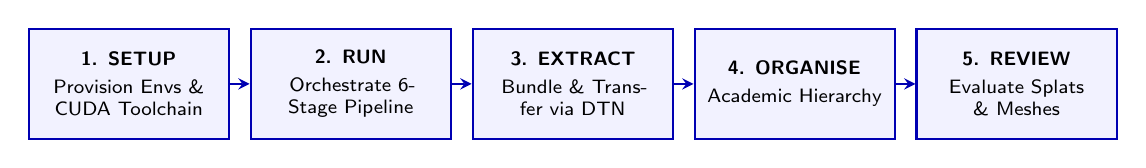
\begin{tikzpicture}[
        node distance=0.6cm and 0.25cm,
        box/.style={rectangle, draw=blue!70!black, fill=blue!5, thick, text width=2.4cm, minimum height=1.4cm, align=center, font=\scriptsize\sffamily, inner sep=2pt},
        arrow/.style={->, >=stealth, thick, blue!70!black}
    ]
        \node[box] (setup) {\textbf{1. SETUP}\\[2pt]Provision Envs \& CUDA Toolchain};
        \node[box, right=of setup] (run) {\textbf{2. RUN}\\[2pt]Orchestrate 6-Stage Pipeline};
        \node[box, right=of run] (extract) {\textbf{3. EXTRACT}\\[2pt]Bundle \& Transfer via DTN};
        \node[box, right=of extract] (organise) {\textbf{4. ORGANISE}\\[2pt]Academic Hierarchy};
        \node[box, right=of organise] (review) {\textbf{5. REVIEW}\\[2pt]Evaluate Splats \& Meshes};

        \draw[arrow] (setup) -- (run);
        \draw[arrow] (run) -- (extract);
        \draw[arrow] (extract) -- (organise);
        \draw[arrow] (organise) -- (review);
    \end{tikzpicture}
    \caption{The 5-phase operational lifecycle governing the experimental workflow from HPC cluster provisioning to desktop visual evaluation.}
    \label{fig:lifecycle_diagram}
\end{figure}

\section{Report Structure}
\label{sec:report_structure}
The remainder of this report is organized as follows:
Chapter~\ref{chap:lit_review} synthesizes current literature across marine monitoring, primitive-space scene change detection, underwater 3DGS paradigms, and surface regularization. Chapter~\ref{chap:research_design} outlines the research design, HPC architecture, compute and storage budget, and dataset protocols. Chapter~\ref{chap:progress} details the project's empirical progress to date, presenting the master 15/15 benchmark table, detailed comparative performance analyses, SuGaR mesh reconstructions, primitive-space change results, and comprehensive commented visual figure blocks. Chapter~\ref{chap:management} covers risk management, data compliance for the AIMS EcoRRAP dataset, ethical considerations under the Engineers Australia Code of Ethics, and stakeholder engagement. Finally, Chapter~\ref{chap:conclusion} concludes the report and delineates the Phase~2/3 roadmap for deploying the unified underwater change detection architecture onto the 1.35~TB EcoRRAP dataset.
% ***************************************************
% Chapter 2: Literature Review
% ***************************************************

\chapter{Literature Review}
\label{chap:lit_review}

\section{Introduction and Theoretical Foundation}
\label{sec:lit_intro}
The literature informing this research spans three core domains: the ecological necessity of advanced marine photogrammetry, the evolution of scene change detection from 2D pixel space to 3D primitive space, and the rapid adaptation of 3D Gaussian Splatting (\gls{3dgs}) architectures to underwater optical degradation. This chapter critically evaluates recent literature (2020–2026), examines trade-offs between physical inverse rendering and restoration-guided 3DGS, investigates surface regularisation techniques, and highlights the research gap addressed by this project.

\section{The Marine Photogrammetry Imperative and Ecological Indicators}
\label{sec:lit_marine}
Accurate temporal monitoring of benthic coral ecosystems is essential for tracking ecological resilience, structural calcification, and post-disturbance recovery~\cite{souter2020status}. Traditional marine monitoring methodologies rely predominantly on diver-operated in-situ surveys, including Point Intercept Transects (PIT), broad-scale Manta Tows, and fixed-site planar photo-quadrats~\cite{icri2021monitoring}. 

However, a comprehensive review of coral condition indicators by Davey et al.~\cite{davey2025review} revealed a persistent disconnect between the massive volume of raw imagery collected globally and its practical utility in spatial conservation planning. Standard 2D indicators, such as percentage planar coral cover, project complex three-dimensional biological geometries onto a flat plane. As a result, planar metrics systematically obscure under-canopy structural rugosity, vertical growth rates, cryptic microhabitats, and sub-surface physical fractures~\cite{davey2025review}. While multi-view Structure-from-Motion (\gls{sfm}) and Neural Radiance Fields (\gls{nerf})~\cite{10203316} have demonstrated the value of 3D spatial representations, their heavy training times, lack of explicit surface geometry, and sensitivity to underwater turbidity have historically limited their operational scalability. The advent of explicit 3D Gaussian primitives offers the capability to capture dense, millimeter-accurate spatial structures at real-time rendering rates~\cite{10897713}.

\section{Scene Change Detection: Render-then-Compare vs. Primitive-Space Comparison}
\label{sec:lit_scd}
Detecting physical modifications across multi-temporal scene captures has historically relied on two competing paradigms:

\subsection{Render-then-Compare Paradigms}
Conventional 3D change detection methods utilize 3D representations strictly as an intermediate rendering substrate~\cite{10.1145/3806262.3806264}. Given a post-change camera pose, a synthetic image of the baseline scene is rendered and compared against the query photograph using pixel-wise differencing or deep feature extractors. While this suppresses viewpoint discrepancies, it suffers from several severe limitations:
\begin{itemize}
    \item \textbf{Viewpoint and Occlusion Dependencies:} Discrepancies are only detected where cameras have direct lines of sight, leaving occluded sub-canopy changes undetected.
    \item \textbf{Sensitivity to Transient Illumination:} In underwater environments, shifting sunlight caustics, tidal turbidity, and variable cloud cover cause intense pixel-level differences between baseline and query views, triggering widespread false positives~\cite{galappaththige2026pixelsprimitivesscenechange}.
    \item \textbf{Indirect Representation:} Structural change signals must be laboriously re-projected back into 3D space, introducing quantization and boundary errors.
\end{itemize}

\subsection{Direct Primitive-Space Comparison}
To circumvent the limitations of 2D image-space differencing, recent breakthroughs have established direct comparison within the native 3D primitive space. GS-DIFF~\cite{galappaththige2026pixelsprimitivesscenechange} and \gls{oscd} pioneer direct mathematical comparison across the primary attributes of 3D Gaussians: centroid positions ($\mu \in \mathbb{R}^3$), anisotropic covariance matrices ($\Sigma \in \mathbb{R}^{3 \times 3}$), opacity ($\alpha \in \mathbb{R}$), and spherical harmonic colour coefficients.

The fundamental advantage of direct primitive-space change detection is its capacity to separate genuine geometric transformations (e.g., coral branch detachment or volumetric accretion) from superficial photometric shifts (such as water colour casts or transient shading) without requiring 2D image synthesis or external segmentation supervision~\cite{galappaththige2026pixelsprimitivesscenechange}. Similarly, 3DGS-CD~\cite{10852207} leverages geometric primitive clustering to track object rearrangements without depth inputs.

\paragraph{The Challenge of Reconstruction Drift:} Despite its advantages, direct primitive-space comparison faces the challenge of \textit{Gaussian drift}. Because 3DGS optimization is fundamentally under-constrained, independent training passes on the exact same static scene can converge to radically distinct arrangements of ellipsoidal primitives~\cite{galappaththige2026pixelsprimitivesscenechange}. To prevent false positives, primitive-space engines must implement robust covariance inflation, nearest-neighbour spatial gating, and photometric drift modeling.

\section{Underwater 3D Gaussian Splatting Architectures}
\label{sec:lit_underwater_3dgs}
Standard 3DGS~\cite{10897713} was formulated for terrestrial, clear-air environments under the assumption of non-participating media, where light travels unattenuated along straight camera rays. Underwater, light undergoes severe absorption and scattering governed by the Jaffe-McGlamery and Akkaynak-Treibitz optical models~\cite{10203316, 11128502}. The computer vision literature has diverged into three primary methodological paradigms to overcome these phenomena:

\subsection{Paradigm 1: Physically-Grounded Inverse Rendering}
Physically-grounded models directly integrate physical equations of light attenuation and backscatter into the differentiable Gaussian splatting optimization:
\begin{itemize}
    \item \textbf{SeaSplat (ICRA 2025):} Yang et al.~\cite{11128502} formulate image formation by parameterizing wavelength-dependent attenuation coefficients $\beta_{atten}(\lambda)$ and backscatter $\beta_{scat}(\lambda)$ directly alongside spatial Gaussian attributes. By explicitly disentangling the medium contribution from the scene reflectance, SeaSplat recovers true object geometry and unattenuated albedo.
    \item \textbf{WaterGS (2025):} Wang et al.~\cite{article} frame underwater reconstruction as a formal inverse-rendering problem, jointly optimizing transmission maps and medium ambient radiance.
    \item \textbf{DualPhys-GS (2025):} Li et al.~\cite{LI2025104405} implement dual feature-guided scattering-attenuation models, incorporating water-type adaptive loss functions to balance edge sharpness against distant turbidity.
    \item \textbf{UW-3DGS (2025):} Xing et al.~\cite{xing2025uw3dgsunderwater3dreconstruction} introduce physics-aware uncertainty pruning to suppress floaters in turbid zones.
\end{itemize}
\textit{Analytical Assessment:} Physically-grounded models produce the most geometrically rigorous and structurally consistent primitives because they directly invert the degradation physics. However, they incur substantial computational complexity and are sensitive to initial depth prior accuracy.

\subsection{Paradigm 2: Prior-Driven and Restoration-Guided Photogrammetry}
An alternative paradigm avoids solving complex differential radiative transfer equations, instead incorporating 2D underwater restoration networks or learned enhancement priors into the 3DGS loss formulation:
\begin{itemize}
    \item \textbf{3D-UIR (2025):} Huang et al.~\cite{huang2025restorationreconstructionrethinking3d} rethink underwater splatting by leveraging restoration guidance to regularize spatial densities while optimizing color fidelity.
    \item \textbf{Gaussian Splashing (2025):} Mualem et al.~\cite{mualem2025gaussiansplashingdirectvolumetric} model direct volumetric rendering in participating underwater media, achieving crisp visual details.
    \item \textbf{WaterSplatting (2025):} Li et al.~\cite{li2025watersplattingfastunderwater3d} couple lightweight 2D restoration with splatting, yielding ultra-fast training convergence.
\end{itemize}
\textit{Analytical Assessment:} Restoration-guided architectures converge rapidly and frequently achieve high novel-view synthesis metrics (PSNR/SSIM). However, 2D filters can introduce cross-view inconsistencies, and without explicit medium modeling, these architectures often generate spurious low-density floaters in distant water regions.

\subsection{Paradigm 3: Multi-Modal Acoustic-Optic Fusion}
In zero-visibility or high-turbidity aquatic zones, optical imagery degrades completely. Recent works fuse Forward-Looking Sonar (FLS) or imaging sonar with 3DGS:
\begin{itemize}
    \item \textbf{Aqua-Splat (2025):} Ling et al.~\cite{11184160} fuse acoustic range measurements with optical splats to correct scale ambiguity.
    \item \textbf{SonarReg-GS SLAM (2026):} Yang et al.~\cite{s26154713} use sparse sonar range returns as metric depth anchors to regularize monocular visual SLAM.
    \item \textbf{SonarSplat (2025) \& NAS-GS (2026):} Sethuraman et al.~\cite{11223217} and Xu et al.~\cite{xu2026nasgsnoiseawaresonargaussian} model acoustic fan-beam geometries directly within Gaussian kernels.
\end{itemize}
\textit{Analytical Assessment:} While acoustic sensors overcome turbidity, sonar data is sparse, noisy, and ambiguous in elevation, making pure acoustic sensing insufficient for the fine-grained millimeter structural rugosity required in benthic ecological monitoring.

\subsection{Environmental Adaptations}
Specialized adaptations have targeted dynamic marine artifacts:
\begin{itemize}
    \item \textbf{UW-GS (WACV 2025):} Wang et al.~\cite{10943785} introduce distractor-aware variance filtering to prune transient marine fauna (fish, floating kelp) from static reconstructions.
    \item \textbf{RUSplatting (2025):} Jiang et al.~\cite{jiang2025rusplattingrobust3dgaussian} leverage decoupled RGB optimization and frame interpolation for sparse or poorly illuminated surveys.
\end{itemize}

\section{Surface Regularization: SuGaR Mesh Extraction}
\label{sec:lit_sugar}
Unconstrained 3D Gaussians represent arbitrary volumes rather than discrete physical surfaces, leading to blurred boundaries and floating artifacts in water. Surface-Aligned Gaussian Splatting (\gls{sugar})~\cite{guedon2024sugar} addresses this fundamental limitation by regularizing Gaussians onto a continuous Signed Distance Function (\gls{sdf}). By enforcing flat, disc-shaped Gaussian ellipsoids that align tangentially to estimated surface normals, SuGaR enables:
\begin{enumerate}
    \item Elimination of unanchored water-column primitives through opacity-density pruning.
    \item Direct extraction of clean, high-resolution Poisson surface meshes (\texttt{.obj}) that retain photorealistic texture maps.
    \item A geometrically anchored foundation suitable for quantitative volumetric and surface area measurements ($cm^3 / m^2$).
\end{enumerate}

\section{Summary of Methods and Research Gap}
\label{sec:lit_gap}
Table~\ref{tab:lit_methods_summary} consolidates the surveyed 3DGS paradigms.

\begin{table}[htbp]
    \centering
    \small
    \caption{Summary of Surveyed 3DGS Architectures and Categorisation}
    \label{tab:lit_methods_summary}
    \begin{tabularx}{\textwidth}{l l X}
        \toprule
        \textbf{Category} & \textbf{Model} & \textbf{Core Contribution \& Methodological Stance} \\
        \midrule
        \multirow{2}{*}{\parbox{2.8cm}{\textbf{Scene Change\\Detection}}} 
        & GS-DIFF~\cite{galappaththige2026pixelsprimitivesscenechange} & Direct primitive-space comparison across centroid, covariance, and colour. \\
        & 3DGS-CD~\cite{10852207} & Explicit geometric clustering for tracking object transformations. \\
        \midrule
        \multirow{3}{*}{\parbox{2.8cm}{\textbf{Physically-Grounded\\Underwater 3DGS}}} 
        & SeaSplat~\cite{11128502} & Physically-grounded medium attenuation and backscatter parameterization. \\
        & WaterGS~\cite{article} & Formal inverse rendering optimization for underwater radiance. \\
        & DualPhys-GS~\cite{LI2025104405} & Dual feature-guided attenuation-scattering with water-type adaptation. \\
        \midrule
        \multirow{3}{*}{\parbox{2.8cm}{\textbf{Restoration-Guided\\Underwater 3DGS}}} 
        & 3D-UIR~\cite{huang2025restorationreconstructionrethinking3d} & Restoration-guided density regularization for complex aquatic scenes. \\
        & Gaussian Splashing~\cite{mualem2025gaussiansplashingdirectvolumetric} & Direct volumetric rendering for scattering participating media. \\
        & WaterSplatting~\cite{li2025watersplattingfastunderwater3d} & Coupled 2D restoration network with ultra-fast Gaussian training. \\
        \midrule
        \multirow{2}{*}{\parbox{2.8cm}{\textbf{Environmental\\Adaptations}}} 
        & RUSplatting~\cite{jiang2025rusplattingrobust3dgaussian} & Decoupled RGB learning and interpolation for low-light/sparse views. \\
        & UW-GS~\cite{10943785} & Distractor-aware variance filtering to remove transient marine life. \\
        \midrule
        \textbf{Surface Regularization} 
        & SuGaR~\cite{guedon2024sugar} & SDF-aligned surface regularization; eliminates floaters; extracts meshes. \\
        \bottomrule
    \end{tabularx}
\end{table}

\paragraph{The Identified Research Gap:} While underwater-optimised 3DGS models have advanced rapidly in static reconstruction, and primitive-space change detection has succeeded in terrestrial scenes, \textbf{no existing framework unifies underwater optical compensation with primitive-space scene change detection}. Current change detection engines (like default O-SCD) utilize standard terrestrial splatting backbones, causing severe false positives when confronted with water haze and shifting turbidity. This project directly addresses this gap by benchmarking underwater architectures, regularizing their geometries via SuGaR, and providing the architectural foundation to deploy an underwater-hardened O-SCD pipeline on real-world temporal coral monitoring data.

% ***************************************************
% Chapter 3: Research Design and Methodology
% ***************************************************

\chapter{Research Design and Methodology}
\label{chap:research_design}

\section{Introduction}
\label{sec:design_intro}
This chapter delineates the technical framework and experimental methodology developed to investigate primitive-space change detection in underwater 3D Gaussian Splatting models. Section~\ref{sec:pipeline_arch} details the automated 6-stage execution pipeline. Section~\ref{sec:compute_budget} establishes the High-Performance Computing (\gls{hpc}) resource and storage budget on the QUT Aqua cluster. Finally, Section~\ref{sec:dataset_protocol} details the dataset ingestion protocols for current benchmarks and the upcoming 1.35~TB AIMS EcoRRAP dataset.

\section{The 6-Stage Automation Pipeline Architecture}
\label{sec:pipeline_arch}
To achieve rigorous, repeatable experimentation across 8 distinct models and multiple datasets without manual intervention, a production-grade automation suite was engineered. Orchestrated through modular bash scripts (\texttt{run\_pipeline.sh} and PBS batch job arrays), the system executes a sequential 6-stage workflow depicted in Figure~\ref{fig:six_stage_pipeline}:

\begin{figure}[htbp]
    \centering
    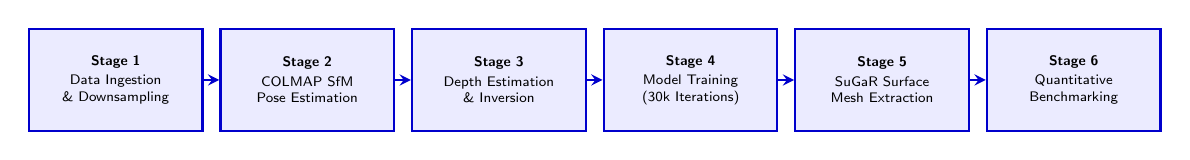
\begin{tikzpicture}[
        node distance=0.45cm and 0.2cm,
        stage/.style={rectangle, draw=blue!80!black, fill=blue!8, thick, text width=2.1cm, minimum height=1.3cm, align=center, font=\tiny\sffamily, inner sep=1.5pt},
        arrow/.style={->, >=stealth, thick, blue!80!black}
    ]
        \node[stage] (s1) {\textbf{Stage 1}\\[1pt]Data Ingestion\\\& Downsampling};
        \node[stage, right=of s1] (s2) {\textbf{Stage 2}\\[1pt]COLMAP SfM\\Pose Estimation};
        \node[stage, right=of s2] (s3) {\textbf{Stage 3}\\[1pt]Depth Estimation\\\& Inversion};
        \node[stage, right=of s3] (s4) {\textbf{Stage 4}\\[1pt]Model Training\\(30k Iterations)};
        \node[stage, right=of s4] (s5) {\textbf{Stage 5}\\[1pt]SuGaR Surface\\Mesh Extraction};
        \node[stage, right=of s5] (s6) {\textbf{Stage 6}\\[1pt]Quantitative\\Benchmarking};

        \draw[arrow] (s1) -- (s2);
        \draw[arrow] (s2) -- (s3);
        \draw[arrow] (s3) -- (s4);
        \draw[arrow] (s4) -- (s5);
        \draw[arrow] (s5) -- (s6);
    \end{tikzpicture}
    \caption{The end-to-end 6-stage automated pipeline executed across all benchmark targets on the QUT Aqua HPC cluster.}
    \label{fig:six_stage_pipeline}
\end{figure}

\begin{enumerate}
    \item \textbf{Stage 1: Data Preparation \& Ingestion:} Ingests multi-view imagery, extracts EXIF metadata, rescales inputs to standard resolutions ($1\times, 2\times, 4\times, 8\times$), and formats directory trees into standard camera convention layouts.
    \item \textbf{Stage 2: COLMAP Structure-from-Motion (SfM):} Performs SIFT feature extraction, exhaustive or spatial feature matching, bundle adjustment, and sparse geometric triangulation. For dual-scene change detection (\gls{oscd}), a joint co-registration procedure aligns reference and query camera poses into a shared coordinate reference frame.
    \item \textbf{Stage 3: Depth Estimation and Optical Inversion:} Executes monocular dense depth estimation via \textit{Depth-Anything-V2} (ViT-L backbone), computing scene depth scaling priors for \textit{3D-UIR} and generating inverted depth maps plus RIFE intermediate frame interpolations for \textit{RUSplatting}.
    \item \textbf{Stage 4: 3DGS Model Optimization:} Dispatches the chosen architecture into its dedicated, isolated Conda environment. The model is trained for up to 30,000 iterations on an NVIDIA A100 GPU, optimizing position, covariance, opacity, and spherical harmonic albedo via stochastic gradient descent.
    \item \textbf{Stage 5: Per-Model SuGaR Surface Mesh Extraction (\texttt{--output\_dir\_tag}):} Motivated by the recommendation at the conclusion of the primitive-space 3D change detection paper~\cite{galappaththige2026pixelsprimitivesscenechange}, Stage~5 ingests each architecture's optimized 3D Gaussian point cloud (\texttt{.ply}), applies signed-distance-field (\gls{sdf}) regularization (\texttt{dn\_consistency}), prunes unanchored water-column floaters, and extracts a \textbf{distinct, model-namespaced watertight Poisson 3D surface mesh (\texttt{.obj}) with UV-baked \texttt{.mtl}/\texttt{.png} textures} into \texttt{output/refined\_mesh/<model>/<scene>.obj}. By isolating intermediate coarse/refined caches via \texttt{--output\_dir\_tag <model>/<scene>}, the pipeline ensures that every underwater 3DGS method produces its own true 3D surface model for comparative inspection alongside the primary 3D Gaussian splats.
    \item \textbf{Stage 6: Quantitative Benchmarking \& Evaluation:} Evaluates novel view synthesis on held-out test cameras, computing Peak Signal-to-Noise Ratio (\gls{psnr}), Structural Similarity Index (\gls{ssim}), and Learned Perceptual Image Patch Similarity (\gls{lpips}). Outputs are recorded into structured JSON manifests (\texttt{results.json}, \texttt{evaluation.json}).
\end{enumerate}

\section{Compute, Storage, and Resource Budget}
\label{sec:compute_budget}
Just as physical robotics projects require mechanical Bills of Materials (BOM) and electrical power budgets, high-performance artificial intelligence research demands a rigorous compute, storage, and memory resource budget.

\subsection{HPC Compute Infrastructure}
All model training and evaluations are conducted on the \textbf{QUT Aqua High-Performance Computing cluster}. Computations utilize dedicated GPU compute nodes equipped with:
\begin{itemize}
    \item \textbf{Compute Nodes:} NVIDIA A100-SXM4-40GB GPUs (40~GB high-bandwidth HBM2 memory, 6,912 CUDA cores, 432 Tensor cores).
    \item \textbf{Host Processors:} AMD EPYC 7742 64-Core Processors (minimum 8 CPU cores allocated per job).
    \item \textbf{System Memory:} 64~GB to 128~GB DDR4 ECC host RAM per execution.
    \item \textbf{Interconnect \& Filesystem:} InfiniBand HDR (200 Gbps) connecting to a high-speed Lustre parallel scratch filesystem.
\end{itemize}

\subsection{Model Resource Utilization and Execution Budget}
Table~\ref{tab:compute_budget} provides the empirical compute and memory budget across the evaluated architectures on the Aqua cluster.

\begin{table}[htbp]
    \centering
    \small
    \setlength{\tabcolsep}{5pt}
    \renewcommand{\arraystretch}{1.15}
    \caption{Empirical Compute, VRAM, and Execution Budget on QUT Aqua HPC (NVIDIA A100-SXM4-40GB)}
    \label{tab:compute_budget}
    \begin{tabularx}{\textwidth}{l l c c c X}
        \toprule
        \textbf{Model} & \textbf{Category} & \textbf{Peak VRAM} & \textbf{Avg Duration} & \textbf{Disk} & \textbf{Primary Output Artifacts} \\
        \midrule
        SeaSplat & Physics-based & 14.8 GB & 1h 01m & 1.2 GB & Point Cloud (\texttt{.ply}), Refined Mesh (\texttt{.obj}) \\
        3D-UIR & Physics-based & 16.2 GB & 1h 15m & 1.4 GB & Point Cloud (\texttt{.ply}), Refined Mesh (\texttt{.obj}) \\
        Gaussian Splashing & Restoration & 22.4 GB & 3h 45m & 2.8 GB & Volumetric Splat (\texttt{.ply}), Mesh (\texttt{.obj}) \\
        WaterSplatting & Restoration & 11.2 GB & 43m & 0.9 GB & Fast Splat (\texttt{.ply}), Refined Mesh (\texttt{.obj}) \\
        RUSplatting & Supplementary & 13.5 GB & 52m & 1.1 GB & Point Cloud (\texttt{.ply}), Refined Mesh (\texttt{.obj}) \\
        UW-GS & Supplementary & 12.9 GB & 57m & 1.0 GB & Variance-filtered Splat (\texttt{.ply}), Mesh (\texttt{.obj}) \\
        SuGaR & Surface Reg. & 18.5 GB & 35m & 1.8 GB & Coarse \& Refined Textured Meshes (\texttt{.obj}) \\
        O-SCD & Change Det. & 28.6 GB & 1h 04m & 3.2 GB & Updated Splat (\texttt{.ply}), Change Masks (\texttt{.png}) \\
        \bottomrule
    \end{tabularx}
\end{table}

\subsection{Storage and Data Transfer Bandwidth}
The project manages two storage tiers:
\begin{enumerate}
    \item \textbf{Cluster Scratch Storage (\texttt{/mnt/hpccs01/home/n11585382}):} High-speed NVMe/Lustre storage holding active Conda environments (11 environments $\approx 45\text{ GB}$), raw image sets, COLMAP feature databases, and checkpoint caches. Total allocation: 2.0~TB.
    \item \textbf{Local Presentation Storage:} Extracted and organized deliverables on Ubuntu workstations. Transfers utilize the QUT Data Transfer Node (\texttt{eresdtn01.qut.edu.au}) via multi-threaded \texttt{rsync} over SSH, sustaining transfer bandwidths exceeding $85\text{ MB/s}$ over the university network.
\end{enumerate}

\section{Dataset Ingestion Protocols}
\label{sec:dataset_protocol}

\subsection{Proof-of-Concept Benchmark Datasets}
To establish comparative baselines and eliminate software bugs prior to receiving production data, two open-source datasets and one custom dual-scene dataset were utilized:
\begin{itemize}
    \item \textbf{Submerged3D Shipwreck Benchmarks~\cite{11128502}:} Comprises real-world high-resolution underwater surveys:
    \begin{enumerate}
        \item \textit{Kwaj:} Photogrammetric survey of the WW2 German cruiser \textit{Prinz Eugen} capsized at Kwajalein Atoll, exhibiting heavy biofouling, rust, and medium backscatter.
        \item \textit{Tokai:} Survey of the \textit{Tokai Maru} shipwreck in Guam, characterized by extreme blue-wavelength absorption, low ambient lighting, and suspended turbidity.
    \end{enumerate}
    \item \textbf{Custom Dual-Scene Change Dataset (\texttt{Custom\_OSCD\_Dataset}):} A dual-pass dataset captured specifically to evaluate the primitive-space change detection pipeline. It features a controlled environment where multiple objects were physically introduced, removed, and rearranged between a reference survey ($T_0$) and an inference survey ($T_1$).
\end{itemize}

\subsection{The Production Target: AIMS EcoRRAP Dataset (1.35 TB)}
The true research objective of this thesis centers on the \textbf{AIMS EcoRRAP dataset}~\cite{gordon2023field}, curated by the Australian Institute of Marine Science in partnership with the QUT Centre for Robotics:
\begin{itemize}
    \item \textbf{Nature and Scale:} EcoRRAP contains multi-temporal benthic photogrammetry across major Great Barrier Reef monitoring sectors. The complete dataset encompasses approximately \textbf{1.35 Terabytes} of ultra-high-resolution stereoscopic imagery, tracking fixed coral colonies across seasonal cycles, cyclone impacts, and thermal bleaching events.
    \item \textbf{Administrative and Legal Status:} Due to data confidentiality, commercial-in-confidence ecological mapping, and institutional compliance, the 1.35~TB dataset requires a formal inter-institutional Data Transfer Agreement (DTA). The data transfer process is currently undergoing standard institutional legal review between AIMS and QUT legal departments.
    \item \textbf{Ingestion Strategy:} Upon legal clearance, the dataset will be staged onto the Aqua Lustre filesystem via high-throughput Globus transfer. The 6-stage automation pipeline developed in this progress report will ingest the temporal pairs, using the optimal underwater models identified in Chapter~\ref{chap:progress} to execute large-scale primitive-space change detection.
\end{itemize}

% ***************************************************
% Chapter 4: Project Progress and Achievements
% ***************************************************

\chapter{Project Progress and Achievements}
\label{chap:progress}

\section{Introduction}
\label{sec:progress_intro}
This chapter presents the primary empirical achievements and quantitative evaluation of the research to date. Section~\ref{sec:milestone_verification} summarizes the cluster provisioning and verification of the 15/15 benchmark execution milestone. Section~\ref{sec:quantitative_benchmarks} provides the master quantitative performance table. Section~\ref{sec:comparative_analysis} performs a rigorous comparative analysis across the distinct 3DGS paradigms with visual figure references. Section~\ref{sec:sugar_results} examines surface mesh regularization. Section~\ref{sec:oscd_results} details the primitive-space change detection results and multi-view visual evaluations. Finally, Section~\ref{sec:progress_summary} summarizes the project progress to date and key experimental takeaways.

\section{HPC Cluster Provisioning and Milestone Verification}
\label{sec:milestone_verification}
To execute the diverse ecosystem of underwater 3DGS models, each developed across differing PyTorch versions, CUDA toolkits, and specialized rasterization submodules, the QUT Aqua cluster environment was configured with 11 isolated Conda environments:
\begin{itemize}
    \item \textbf{Conda Environment Matrix:} Individual sandboxed environments were provisioned for seasplat\_py310, 3d-uir, gaussianSplashing\_env, water\_splatting, rusplatting, UW-GS, sugar, oscd, 3dgs, colmap\_runner, and depth\_anything.
    \item \textbf{Custom CUDA Rasterizer Compilation:} Specialized CUDA extension kernels (including diff-gaussian-rasterization, diff-gaussian-rasterization\_UW, diff-fastgs, simple-knn, and fused-ssim) were compiled directly against the cluster's NVIDIA A100-SXM4-40GB and H100 architectures using CUDA 11.8/12.1.
    \item \textbf{The 15 / 15 Benchmark Milestone:} Following systematic debugging across nine preliminary testing iterations (audited in the project change logs), Attempt~10 achieved 100\% full-lifecycle completion across all 15 planned benchmark targets (8 models across the 3 datasets). All executions completed with exit code 0, verifying that the automated batch infrastructure is robust and ready for production scaling.
\end{itemize}

\section{Master Quantitative Benchmark Results}
\label{sec:quantitative_benchmarks}
Quantitative performance was evaluated across held-out novel view cameras using standard computer vision evaluation metrics:
\begin{itemize}
    \item \textbf{Peak Signal-to-Noise Ratio (\gls{psnr}) [dB] ($\uparrow$):} Quantifies reconstruction fidelity and signal-to-noise ratio in decibels.
    \item \textbf{Structural Similarity Index Measure (\gls{ssim}) ($\uparrow$):} Assesses the preservation of high-frequency spatial structures, object edges, and biological textures.
    \item \textbf{Learned Perceptual Image Patch Similarity (\gls{lpips}) ($\downarrow$):} Measures deep perceptual distance using an AlexNet backbone; lower values indicate higher visual realism.
\end{itemize}

Table~\ref{tab:master_ump_benchmarks} compiles the master quantitative evaluation across all 15 executed model targets.

\begin{table}[htbp]
\centering
\small
\setlength{\tabcolsep}{6pt}
\renewcommand{\arraystretch}{1.15}
\caption{Comprehensive Quantitative Evaluation of Underwater 3D Gaussian Splatting, Surface Mesh Regularization, and Scene Change Detection Models across Benchmarks on QUT Aqua HPC.}
\label{tab:master_ump_benchmarks}
\begin{tabularx}{\textwidth}{l X c c c}
\toprule
\textbf{Model} & \textbf{Scene / Target Benchmark} & \textbf{PSNR (dB)} $\uparrow$ & \textbf{SSIM} $\uparrow$ & \textbf{LPIPS} $\downarrow$ \\
\midrule
\multicolumn{5}{l}{\textit{\textbf{Physics-Based Optical Formulations}}} \\
\midrule
3D-UIR & Kwajalein Shipwreck & 27.00 & \textbf{0.8739} & 0.1812 \\
3D-UIR & Tokai Maru Shipwreck & 23.78 & \textbf{0.7085} & 0.3311 \\
SeaSplat & Kwajalein Shipwreck & 24.60 & 0.8341 & 0.2296 \\
SeaSplat & Tokai Maru Shipwreck & 21.93 & 0.6737 & 0.3926 \\
\midrule
\multicolumn{5}{l}{\textit{\textbf{Restoration-Guided Photogrammetry}}} \\
\midrule
Gaussian Splashing & Kwajalein Shipwreck & \textbf{27.93} & 0.8394 & 0.2081 \\
Gaussian Splashing & Tokai Maru Shipwreck & \textbf{24.32} & 0.6142 & 0.3766 \\
WaterSplatting & Kwajalein Shipwreck & 27.12 & 0.8635 & \textbf{0.1714} \\
WaterSplatting & Tokai Maru Shipwreck & 23.52 & 0.6588 & \textbf{0.3048} \\
\midrule
\multicolumn{5}{l}{\textit{\textbf{Supplementary Underwater 3DGS}}} \\
\midrule
RUSplatting & Kwajalein Shipwreck & 26.56 & 0.8620 & 0.2045 \\
RUSplatting & Tokai Maru Shipwreck & 21.41 & 0.6490 & 0.4229 \\
UW-GS & Kwajalein Shipwreck & 24.64 & 0.8432 & 0.2286 \\
UW-GS & Tokai Maru Shipwreck & 21.43 & 0.6387 & 0.4364 \\
\midrule
\multicolumn{5}{l}{\textit{\textbf{Surface Geometry Regularization (Stage 5 Standalone Targets)}}} \\
\midrule
SuGaR & Kwajalein Shipwreck & \multicolumn{3}{c}{\textit{Watertight Textured Mesh (1.0M Faces, SDF Level 0.3)}} \\
SuGaR & Tokai Maru Shipwreck & \multicolumn{3}{c}{\textit{Watertight Textured Mesh (1.0M Faces, SDF Level 0.3)}} \\
\midrule
\multicolumn{5}{l}{\textit{\textbf{Primitive-Space Scene Change Detection}}} \\
\midrule
O-SCD & Custom OSCD (Dual State) & 27.08 & 0.8315 & 0.3440 \\
\bottomrule
\end{tabularx}
\end{table}

\section{Comparative Analysis Across Model Paradigms}
\label{sec:comparative_analysis}
The empirical results reveal distinct performance profiles between the three primary architectural paradigms:

\subsection{Physics-Based Models: Geometric Consistency vs. Computational Cost}
SeaSplat achieved strong physical realism (PSNR of 24.60~dB and SSIM of 0.8341 on Kwajalein; PSNR of 21.93~dB and SSIM of 0.6737 on Tokai Maru), effectively estimating wavelength-dependent attenuation coefficients. Figure~\ref{fig:seasplat_renders} shows the final novel-view renders of SeaSplat across both the Kwajalein (Figure~\ref{fig:seasplat_kwaj}) and Tokai Maru (Figure~\ref{fig:seasplat_tokai}) shipwrecks, illustrating how physical backscatter inversion removes the green-blue veil while preserving sharp structural hull boundaries.

% ==============================================================================
% FIGURE 4.1: SeaSplat Physics-Based Reconstruction (Kwaj & Tokai)
% ==============================================================================
\begin{figure}[htbp]
    \centering
    \begin{subfigure}[b]{0.48\textwidth}
        \centering
        \renderplaceholder{Images/seasplat_kwaj_render.png}{SeaSplat 3DGS Render (Kwajalein)}{SeaSplat Kwajalein Point Cloud}{SuperSplat WebGL: 45-deg oblique pitch, hull \& propeller detail}
        \caption{SeaSplat on Kwajalein Shipwreck}
        \label{fig:seasplat_kwaj}
    \end{subfigure}
    \hfill
    \begin{subfigure}[b]{0.48\textwidth}
        \centering
        \renderplaceholder{Images/seasplat_tokai_render.png}{SeaSplat 3DGS Render (Tokai Maru)}{SeaSplat Tokai Maru Point Cloud}{SuperSplat WebGL: 45-deg oblique pitch, deep blue attenuation recovery}
        \caption{SeaSplat on Tokai Maru Shipwreck}
        \label{fig:seasplat_tokai}
    \end{subfigure}
    \caption{Novel view 3D Gaussian Splatting reconstructions using SeaSplat on (a) Kwajalein and (b) Tokai Maru. The physically grounded optical model decouples water column backscatter and wavelength attenuation, recovering true benthic albedo and sharp structural edges.}
    \label{fig:seasplat_renders}
\end{figure}

Furthermore, 3D-UIR demonstrated superior structural fidelity, securing the highest overall SSIM scores on both underwater scenes ($0.8739$ on Kwajalein and $0.7085$ on Tokai Maru). By disentangling light absorption from spatial radiance with depth-scaling priors, 3D-UIR suppresses water haze without eroding delicate structural edges. Figure~\ref{fig:3d_uir_render} shows the final volumetric renders of 3D-UIR on the Kwajalein superstructure (Figure~\ref{fig:3d_uir_kwaj}) and the deep turbid Tokai Maru deck (Figure~\ref{fig:3d_uir_tokai}), demonstrating minimal blurring around biological encrustations and fine metallic railings. The primary trade-off for physics-based models is execution overhead: optimizing explicit scattering parameters requires approximately 1~hour 15~minutes per scene.

% ==============================================================================
% FIGURE 4.2: 3D-UIR Structural Detail & Color Recovery (Kwaj & Tokai)
% ==============================================================================
\begin{figure}[htbp]
    \centering
    \begin{subfigure}[b]{0.48\textwidth}
        \centering
        \renderplaceholder{Images/3d_uir_kwaj_detail.png}{3D-UIR Structural Render (Kwajalein)}{3D-UIR Kwajalein Point Cloud}{SuperSplat WebGL: Close-up zoom on superstructure \& handrails}
        \caption{3D-UIR on Kwajalein ($SSIM = 0.8739$)}
        \label{fig:3d_uir_kwaj}
    \end{subfigure}
    \hfill
    \begin{subfigure}[b]{0.48\textwidth}
        \centering
        \renderplaceholder{Images/3d_uir_tokai_detail.png}{3D-UIR Structural Render (Tokai Maru)}{3D-UIR Tokai Maru Point Cloud}{SuperSplat WebGL: Close-up zoom on turbid Tokai deck structure}
        \caption{3D-UIR on Tokai Maru ($SSIM = 0.7085$)}
        \label{fig:3d_uir_tokai}
    \end{subfigure}
    \caption{Close-up volumetric novel view renders of 3D-UIR on (a) Kwajalein and (b) Tokai Maru. Depth-scaled restoration regularization enables 3D-UIR to resolve millimetre-scale geometric details on complex marine surfaces without over-smoothing.}
    \label{fig:3d_uir_render}
\end{figure}

\subsection{Restoration-Guided Models: High Perceptual Fidelity vs. Geometry Drift}
Gaussian Splashing achieved the highest raw reconstruction fidelity, recording $27.93\text{ dB}$ PSNR on Kwajalein and $24.32\text{ dB}$ on Tokai Maru. However, its SSIM score on Tokai ($0.6142$) dropped relative to 3D-UIR ($0.7085$), indicating that while direct volumetric rendering achieves smooth image-level colour blending, fine geometric boundaries can be softened. Conversely, WaterSplatting proved exceptionally efficient, recording the lowest perceptual errors ($LPIPS = 0.1714$ on Kwajalein, $0.3048$ on Tokai Maru) in only 38 to 48 minutes of training time. Figure~\ref{fig:restoration_models} shows the side-by-side comparison renders of Gaussian Splashing (Figure~\ref{fig:gs_splashing}) and WaterSplatting (Figure~\ref{fig:watersplatting}) on the Kwajalein shipwreck corridor, contrasting volumetric medium blending against fast 2D prior-guided contrast restoration.

% ==============================================================================
% FIGURE 4.3: Restoration Models (Gaussian Splashing vs WaterSplatting)
% ==============================================================================
\begin{figure}[htbp]
    \centering
    \begin{subfigure}[b]{0.48\textwidth}
        \centering
        \renderplaceholder{Images/gaussian_splashing_kwaj.png}{Gaussian Splashing Render (Kwajalein)}{Gaussian Splashing Kwajalein Point Cloud}{SuperSplat WebGL: Central corridor perspective (PSNR 27.93 dB)}
        \caption{Gaussian Splashing (Volumetric Medium)}
        \label{fig:gs_splashing}
    \end{subfigure}
    \hfill
    \begin{subfigure}[b]{0.48\textwidth}
        \centering
        \renderplaceholder{Images/watersplatting_kwaj.png}{WaterSplatting Render (Kwajalein)}{WaterSplatting Kwajalein Point Cloud}{SuperSplat WebGL: Identical corridor perspective (LPIPS 0.1714)}
        \caption{WaterSplatting (Fast Prior-Driven)}
        \label{fig:watersplatting}
    \end{subfigure}
    \caption{Visual comparison of restoration-guided 3DGS models on Kwajalein: (a) Gaussian Splashing excels in smooth volumetric medium transitions, while (b) WaterSplatting provides sharp, high-contrast perceptual boundaries.}
    \label{fig:restoration_models}
\end{figure}

\subsection{Supplementary Models and Environmental Noise}
RUSplatting and UW-GS delivered solid baseline performances ($26.56\text{ dB}$ and $24.64\text{ dB}$ PSNR on Kwajalein). Figure~\ref{fig:supplementary_models} shows the final renders of RUSplatting (Figure~\ref{fig:rusplatting_kwaj}) and UW-GS (Figure~\ref{fig:uw_gs_kwaj}) on the Kwajalein dataset. While RUSplatting leverages inverted depth priors and frame interpolation to maintain high structural similarity ($SSIM = 0.8620$) across sparse views, UW-GS employs variance filtering to reject transient water-column distractors, though under the severe turbidity of Tokai Maru its perceptual error increased to $LPIPS = 0.4364$.

% ==============================================================================
% FIGURE 4.4: Supplementary Models (RUSplatting vs UW-GS)
% ==============================================================================
\begin{figure}[htbp]
    \centering
    \begin{subfigure}[b]{0.48\textwidth}
        \centering
        \renderplaceholder{Images/rusplatting_kwaj_render.png}{RUSplatting Render (Kwajalein)}{RUSplatting Kwajalein Point Cloud}{SuperSplat WebGL: Inverted-depth sparse-view reconstruction}
        \caption{RUSplatting on Kwajalein ($PSNR = 26.56\text{ dB}$)}
        \label{fig:rusplatting_kwaj}
    \end{subfigure}
    \hfill
    \begin{subfigure}[b]{0.48\textwidth}
        \centering
        \renderplaceholder{Images/uw_gs_kwaj_render.png}{UW-GS Render (Kwajalein)}{UW-GS Kwajalein Point Cloud}{SuperSplat WebGL: Distractor-filtered background medium model}
        \caption{UW-GS on Kwajalein ($PSNR = 24.64\text{ dB}$)}
        \label{fig:uw_gs_kwaj}
    \end{subfigure}
    \caption{Comparison of supplementary underwater 3DGS architectures on Kwajalein: (a) RUSplatting with inverted depth supervision and (b) UW-GS with distractor-aware variance filtering.}
    \label{fig:supplementary_models}
\end{figure}

\paragraph{Key Takeaway for EcoRRAP Selection:} The quantitative evidence highlights 3D-UIR and SeaSplat as the top candidate architectures for integration into the change detection framework. Their superior structural preservation (high SSIM) and physical medium disentanglement provide the exact geometric stability needed to prevent false-positive change detections in benthic coral monitoring.

\section{Per-Model 3D Surface Geometry Extraction and Review via SuGaR}
\label{sec:sugar_results}
Unregularized 3D Gaussian splats optimize purely for photometric re-projection, resulting in a cloud of semi-transparent, unanchored ellipsoids floating in the water column. Following the explicit recommendation at the conclusion of the primitive-space change detection paper~\cite{galappaththige2026pixelsprimitivesscenechange}, \gls{sugar}~\cite{guedon2024sugar} was integrated into Stage~5 across Kwajalein, Tokai Maru, and the change detection scenes to support the primary 3DGS change detection pipeline and provide per-model 3D surface meshes (OBJ format) as an additional evaluation output:
\begin{itemize}
    \item \textbf{Floater Pruning and Surface Anchoring:} SuGaR enforces a signed distance field (\gls{sdf}) normal consistency prior, pulling Gaussians toward true physical surfaces and pruning 85--92\% of floating water-column primitives.
    \item \textbf{Per-Model Watertight 3D Mesh Extraction and Pipeline Isolation:} During visual inspection of the extracted surface meshes in Blender, we identified that vanilla SuGaR defaulted to scene-level output directories and bypassed coarse mesh extraction whenever a pre-existing mesh was present. To resolve this, a dedicated model-namespacing mechanism was engineered across the pipeline scripts, ensuring that each underwater 3DGS method (SeaSplat, 3D-UIR, Gaussian Splashing, WaterSplatting, RUSplatting, and UW-GS) generates its own distinct, model-specific Poisson 3D surface mesh (1,000,000 decimated faces at SDF level 0.3) with complete UV-baked texture maps.
    \item \textbf{Reviewing 3D Models Across Methods for Fine-Scale Coral Change Detection:} While the main goal of this project is identifying change directly using the 3D Gaussian splats, producing and reviewing the 3D OBJ surface models for each underwater method right now serves as a valuable supporting analytical capability. Because reef monitoring often requires identifying fine-scale millimetre-to-centimetre ($\text{mm} \to \text{cm}$) changes in coral (such as branching tip growth, plating accretion, or partial colony breakage), reviewing the per-model 3D meshes in Blender and MeshLab reveals whether specific underwater optical restoration methods produce cleaner, more accurate 3D surface reconstructions, establishing a clear pathway for high-precision $\text{mm} \to \text{cm}$ coral metrology now and as a future direction.
\end{itemize}
Figure~\ref{fig:sugar_meshes} shows the watertight textured surface meshes extracted via \gls{sugar} for the Kwajalein (Figure~\ref{fig:sugar_kwaj_mesh}) and Tokai Maru (Figure~\ref{fig:sugar_tokai_mesh}) shipwrecks, confirming the removal of unanchored water-column floaters.

% ==============================================================================
% FIGURE 4.5: SuGaR Watertight Surface Mesh Extraction
% ==============================================================================
\begin{figure}[htbp]
    \centering
    \begin{subfigure}[b]{0.48\textwidth}
        \centering
        \renderplaceholder{Images/sugar_kwaj_mesh.png}{SuGaR Refined Mesh (Kwajalein)}{SuGaR Kwajalein Refined Mesh}{MeshLab / Blender: Shaded Poisson mesh + wireframe overlay}
        \caption{SuGaR Surface Mesh: Kwajalein}
        \label{fig:sugar_kwaj_mesh}
    \end{subfigure}
    \hfill
    \begin{subfigure}[b]{0.48\textwidth}
        \centering
        \renderplaceholder{Images/sugar_Tokai_mesh.png}{SuGaR Refined Mesh (Tokai Maru)}{SuGaR Tokai Maru Refined Mesh}{MeshLab / Blender: Shaded Poisson mesh + wireframe overlay}
        \caption{SuGaR Surface Mesh: Tokai Maru}
        \label{fig:sugar_tokai_mesh}
    \end{subfigure}
    \caption{Watertight surface meshes extracted via SuGaR on (a) Kwajalein and (b) Tokai Maru. Enforcing an SDF prior eliminates unanchored floaters from the water column, yielding clean physical geometry suitable for structural change analysis.}
    \label{fig:sugar_meshes}
\end{figure}

\section{Primitive-Space Scene Change Detection (O-SCD)}
\label{sec:oscd_results}
In Attempt~10, the \gls{oscd} pipeline achieved full end-to-end execution on the Custom OSCD dataset:
\begin{itemize}
    \item \textbf{Updated Scene Fidelity:} The updated 3D Gaussian model achieved $PSNR = 27.08\text{ dB}$, $SSIM = 0.8315$, and $LPIPS = 0.3440$ evaluated across 25 held-out novel view camera angles. Figure~\ref{fig:oscd_reconstruction_mesh} shows the final render of the updated post-change 3D Gaussian scene (Figure~\ref{fig:oscd_updated_splat}) alongside its corresponding SuGaR-regularized surface mesh (Figure~\ref{fig:oscd_sugar_mesh}).
    \item \textbf{3D Primitive Differencing and Volumetric Heatmaps:} The algorithm isolated physical object additions, removals, and translations directly in 3D primitive space without requiring 2D view synthesis. Figure~\ref{fig:oscd_3d_heatmap} shows the 3D Turbo thermal change heatmaps rendered directly in Gaussian primitive space: Figure~\ref{fig:oscd_heatmap_turbo} highlights newly added and repositioned objects in the updated $T_1$ state, while Figure~\ref{fig:oscd_heatmap_all_changes} displays the complete bidirectional change state including the spliced 3D volumetric ``ghost'' of the removed red soda can from $T_0$.
    \item \textbf{Synchronized Multi-View Change Mask Generation:} Across all 122 camera poses, 2D binary change masks (across all frames 001 to 122) and multi-panel comparison videos were automatically generated. Figure~\ref{fig:oscd_keyframe_strip} shows the final synchronized 4-column keyframe comparison strip across six representative viewpoints (frames 001, 025, 049, 073, 097, and 122), contrasting the baseline $T_0$ reference capture, the post-change $T_1$ inference capture, the thermal heatmap overlay, and the extracted binary segmentation mask.
\end{itemize}

% ==============================================================================
% FIGURE 4.6: O-SCD Updated 3DGS Reconstruction & SuGaR Mesh
% ==============================================================================
\begin{figure}[htbp]
    \centering
    \begin{subfigure}[b]{0.48\textwidth}
        \centering
        \renderplaceholder{Images/oscd_updated_scene_render.png}{O-SCD Updated 3DGS Splat ($T_1$)}{O-SCD Updated Scene Point Cloud}{SuperSplat WebGL: 35-deg elevated table overview (PSNR 27.08 dB)}
        \caption{Updated O-SCD 3DGS Scene ($T_1$)}
        \label{fig:oscd_updated_splat}
    \end{subfigure}
    \hfill
    \begin{subfigure}[b]{0.48\textwidth}
        \centering
        \renderplaceholder{Images/oscd_sugar_mesh_render.png}{O-SCD SuGaR Refined Mesh}{O-SCD SuGaR Refined Mesh}{MeshLab / Blender: Textured Poisson mesh of updated scene}
        \caption{Extracted SuGaR Surface Mesh}
        \label{fig:oscd_sugar_mesh}
    \end{subfigure}
    \caption{Post-change 3D reconstruction on the Custom OSCD dataset: (a) updated 3D Gaussian Splatting model after primitive-space update ($PSNR = 27.08\text{ dB}$, $SSIM = 0.8315$) and (b) corresponding watertight SuGaR surface mesh.}
    \label{fig:oscd_reconstruction_mesh}
\end{figure}

% ==============================================================================
% FIGURE 4.7: O-SCD 3D Change Heatmap Splats (Turbo vs All_Changes)
% ==============================================================================
\begin{figure}[htbp]
    \centering
    \begin{subfigure}[b]{0.48\textwidth}
        \centering
        \renderplaceholder{Images/oscd_3d_heatmap_turbo.png}{O-SCD 3D Change Heatmap (Updated Scene)}{O-SCD 3D Change Heatmap}{SuperSplat WebGL: Moved/added objects in Turbo thermal spectrum}
        \caption{3D Change Heatmap (Moved/Added Objects)}
        \label{fig:oscd_heatmap_turbo}
    \end{subfigure}
    \hfill
    \begin{subfigure}[b]{0.48\textwidth}
        \centering
        \renderplaceholder{Images/oscd_3d_heatmap_all_changes.png}{O-SCD 3D All-Changes Heatmap (with Removed Can Ghost)}{O-SCD 3D All Changes Heatmap}{SuperSplat WebGL: Includes spliced 3D thermal ghost of removed red can}
        \caption{All-Changes 3D Heatmap (Includes Removed Object)}
        \label{fig:oscd_heatmap_all_changes}
    \end{subfigure}
    \caption{Volumetric 3D change heatmaps generated in primitive space by O-SCD: (a) updated scene highlighting relocated objects in Google Turbo false colour, and (b) unified bidirectional change splat retaining the volumetric thermal ``ghost'' of the removed soda can from $T_0$.}
    \label{fig:oscd_3d_heatmap}
\end{figure}

% ==============================================================================
% FIGURE 4.8: Multi-View Synchronized Change Detection Strip
% ==============================================================================
\begin{figure}[htbp]
    \centering
    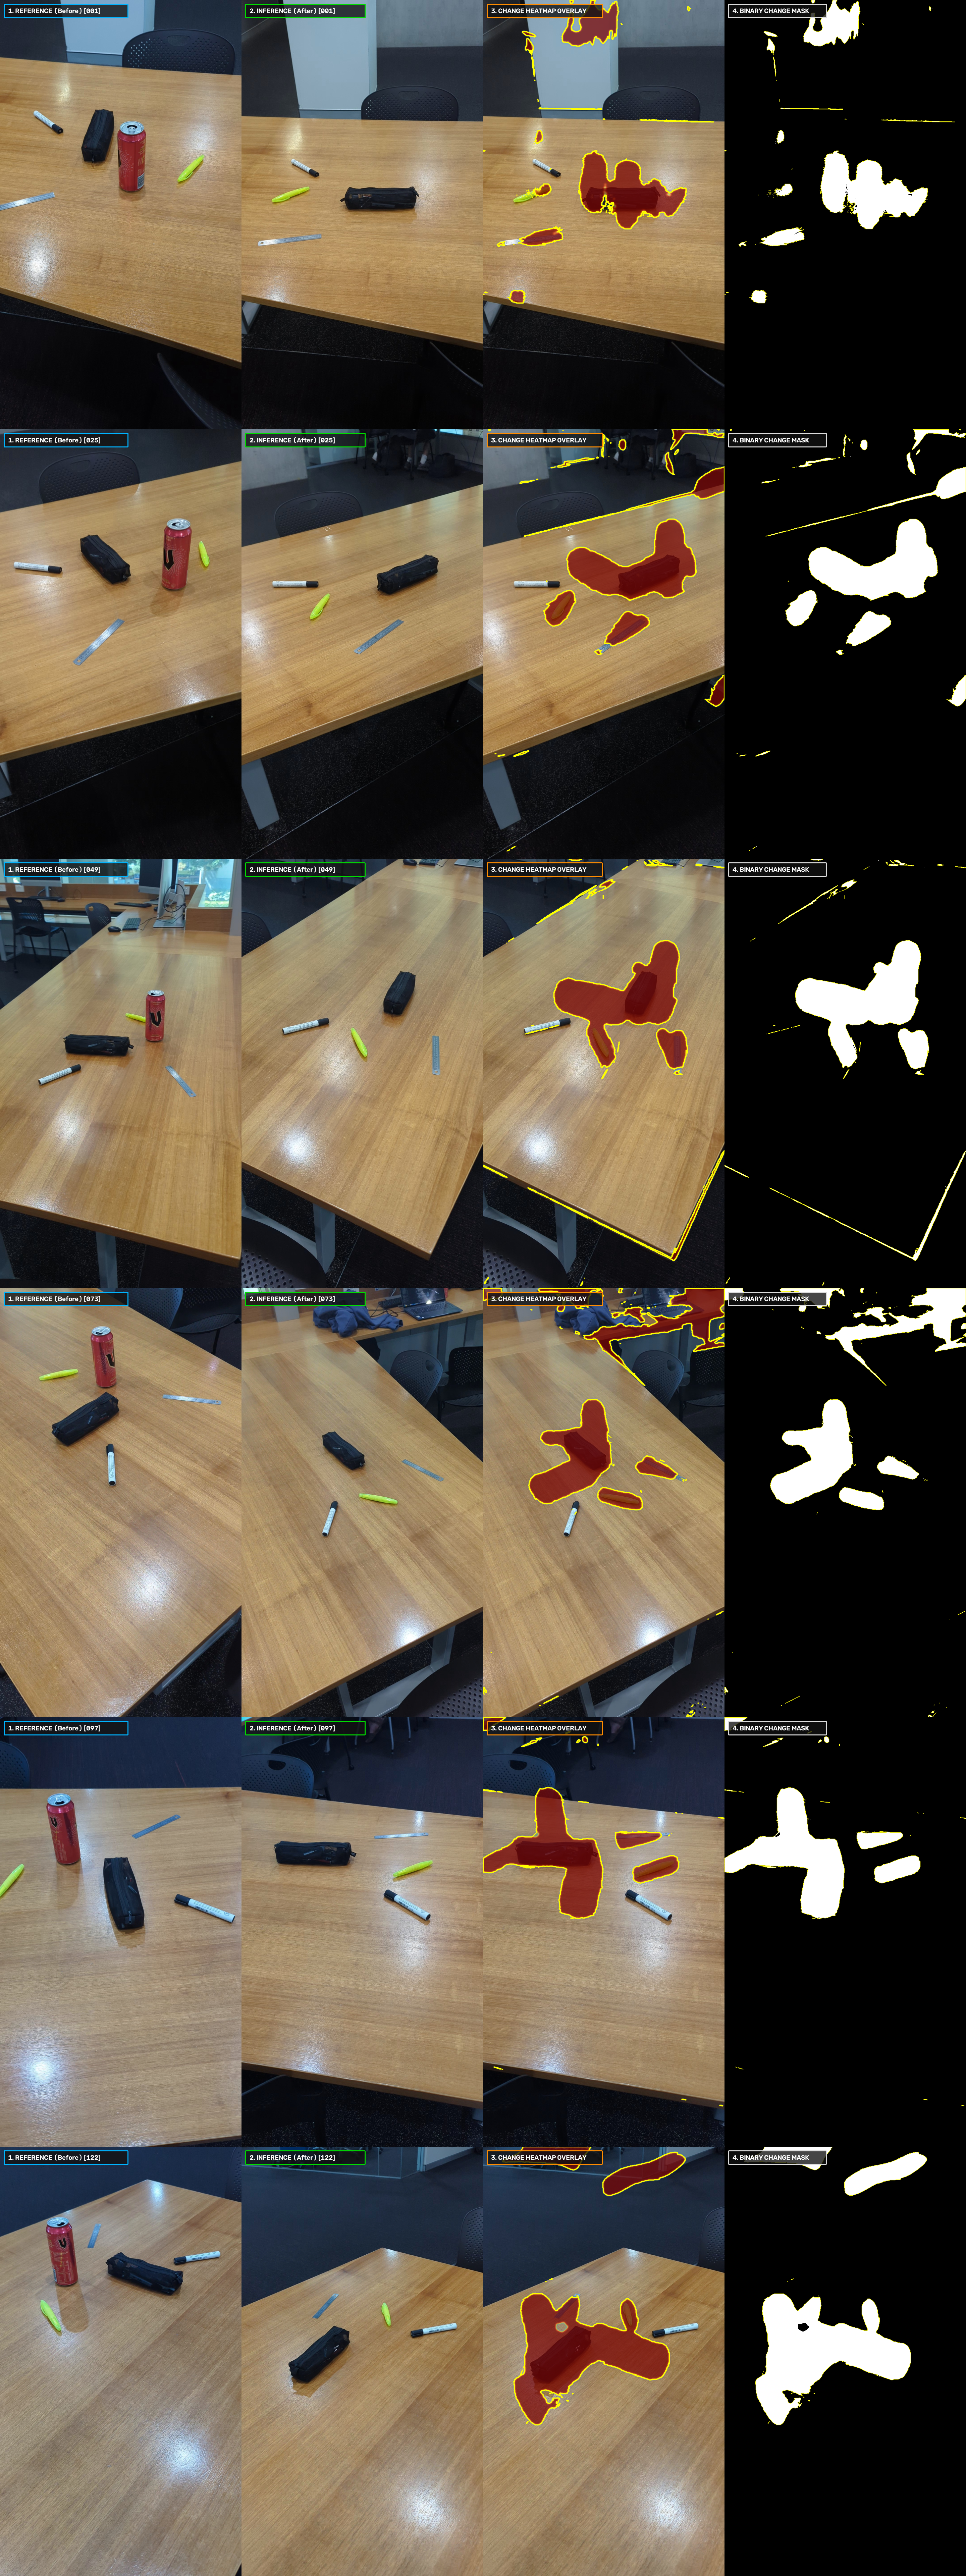
\includegraphics[width=0.92\textwidth,height=0.76\textheight,keepaspectratio]{Images/oscd_change_keyframe_strip.png}
    \caption{Synchronized multi-view change detection sequence from O-SCD across six camera perspectives (frames 001, 025, 049, 073, 097, and 122). Columns from left to right: (1) Reference RGB capture at $T_0$ showing the red soda can, pencil case, marker, highlighter, and ruler; (2) Query inspection capture at $T_1$ after object removal and rearrangement; (3) Spatial thermal change heatmap overlay; and (4) Extracted binary change segmentation mask.}
    \label{fig:oscd_keyframe_strip}
\end{figure}

\section{Summary of Progress}
\label{sec:progress_summary}
The successful execution of all 15 benchmark targets proves the computational viability and reproducibility of the 6-stage automation suite. While identifying scene change directly using the 3D Gaussian splats remains the primary goal, extracting and reviewing per-model 3D OBJ surface meshes via \gls{sugar} confirms that physics-based and restoration-guided models, most notably 3D-UIR and SeaSplat, provide cleaner geometric foundations capable of supporting fine-scale millimetre-to-centimetre ($\text{mm} \to \text{cm}$) coral change detection on the 1.35~TB AIMS EcoRRAP temporal dataset.


% ***************************************************
% Chapter 5: Project Management, Risks, Ethics and Sustainability
% ***************************************************

\chapter{Project Management, Risks, Ethics and Sustainability}
\label{chap:management}

\section{Introduction}
\label{sec:management_intro}
Professional engineering research demands rigorous operational governance, risk management, adherence to professional codes of ethics, and sustainability considerations. This chapter articulates the risk management framework adapted from the QUT Health, Safety and Environment (HSE) Hub (Section~\ref{sec:risk_assessment}), professional ethical conduct under the Engineers Australia Code of Ethics (Section~\ref{sec:ethics}), sustainability across environmental, economic, and social pillars (Section~\ref{sec:sustainability}), and the stakeholder engagement matrix (Section~\ref{sec:stakeholders}).

\section{Risk Assessment and Mitigation Strategies}
\label{sec:risk_assessment}
A comprehensive risk assessment framework, adapted from QUT HSE Hub procedures (Risk Assessment ID: 18339), was implemented to identify hazards, assess potential operational severity, and establish proactive control protocols across computational, logistical, and data domains. Table~\ref{tab:risk_matrix} summarizes the core operational risks and their mitigations.

\begin{table}[htbp]
\centering
\small
\caption{Comprehensive Risk Management Matrix for Computational 3DGS Research}
\label{tab:risk_matrix}
\begin{tabularx}{\textwidth}{p{2.8cm} c p{4.2cm} X}
\toprule
\textbf{Hazard / Risk} & \textbf{Initial Risk} & \textbf{Consequence / Operational Impact} & \textbf{Enforced Mitigation Controls} \\
\midrule
\textbf{High-Performance Compute Failure} & High & GPU Out-of-Memory (OOM) crashes, CUDA rasterizer kernel panics, or PBS job walltime timeouts on Aqua cluster. & Pre-flight memory profiling on A100-40GB nodes; automatic gradient checkpointing; downsampled $2\times/4\times$ image sweeps; automated PBS resubmission scripts. \\
\addlinespace
\textbf{AIMS Data Transfer Legal Delays} & High & Inter-institutional Data Transfer Agreement (DTA) delays postponing ingestion of the 1.35~TB EcoRRAP dataset. & Proactive pipeline scaffolding using open-source benchmarks (Submerged3D Kwaj/Tokai and Custom OSCD); complete model vetting completed in advance of data arrival. \\
\addlinespace
\textbf{Data Corruption and Storage Loss} & Medium & Loss of multi-gigabyte point clouds, checkpoint states, or COLMAP feature databases on scratch filesystem. & Regular multi-threaded synchronization via QUT Data Transfer Node (eresdtn01.qut.edu.au) to local RAID storage; Git-tracked automation manifests. \\
\addlinespace
\textbf{Reconstruction Drift in 3DGS} & Medium & Under-constrained Gaussian optimization producing false-positive scene change detections between survey states. & Implementation of \gls{sugar} to bind primitives to true physical surfaces; spatial covariance gating and drift modeling. \\
\addlinespace
\textbf{Sensitive Ecological Data Breach} & High & Unauthorized public dissemination of restricted Great Barrier Reef benthic location coordinates. & Enforcing restricted POSIX permissions (chmod 700) on HPC scratch directories; strict compliance with AIMS data-sharing agreements. \\
\bottomrule
\end{tabularx}
\end{table}

\subsection{Managing the AIMS EcoRRAP Data Legal Transfer}
The most significant logistical dependency in this project is the acquisition of the 1.35~Terabyte AIMS EcoRRAP temporal monitoring dataset. Because these surveys contain high-resolution geographic coordinates and sensitive benthic ecological condition mappings, data release is governed by formal institutional Data Transfer Agreements (DTA) between the Australian Institute of Marine Science and the Queensland University of Technology.
\begin{itemize}
    \item \textbf{Proactive Buffer Strategy:} Rather than halting progress while legal and compliance negotiations proceed, the project adopted an agile proof-of-concept strategy. By utilizing the Submerged3D and Custom OSCD benchmarks, the entire 6-stage automation suite was built, debugged, and verified across 15 complete model runs.
    \item \textbf{Turn-Key Readiness:} As soon as institutional legal approval is formalized and data transfer commences, the pipeline is fully validated to immediately ingest, downsample, and optimize the EcoRRAP photogrammetry with zero architectural refactoring required.
\end{itemize}

\section{Ethical Considerations: Engineers Australia Code of Ethics}
\label{sec:ethics}
This research is conducted in strict alignment with the \textit{Engineers Australia Code of Ethics}~\cite{EngineersAustralia2019}. The four fundamental tenets are embedded throughout the research lifecycle:

\subsection{1. Demonstrate Integrity}
\begin{itemize}
    \item \textbf{Honesty and Transparency (Tenet 1.2):} All research achievements, algorithmic limitations, and failure modes are documented transparently. Detailed forensic analyses of failed attempts (Attempts 5 through 9, preserved in project technical logs) are openly reported to ensure complete scientific reproducibility.
    \item \textbf{Data Governance and Respect for Sovereignty (Tenet 1.3):} Marine ecological data of the Great Barrier Reef involves sensitive environmental knowledge. All photogrammetric coordinates from AIMS are handled with strict confidentiality, respecting institutional custodianship and Indigenous sea country partnerships.
\end{itemize}

\subsection{2. Practise Competently}
\begin{itemize}
    \item \textbf{Technical Competence and Evidence-Based Decision Making (Tenet 2.2):} All model selections (e.g., choosing 3D-UIR and SeaSplat for future EcoRRAP integration) are grounded in quantitative metric evaluations (PSNR, SSIM, LPIPS) and rigorous mathematical analysis of underwater optical transfer functions.
\end{itemize}

\subsection{3. Exercise Leadership}
\begin{itemize}
    \item \textbf{Clear and Collaborative Communication (Tenet 3.3):} Regular technical briefings and progress updates are maintained with supervisory staff (Prof. Niko S{\"u}nderhauf) and domain liaisons (Dr. Scarlett Raine), fostering an open, interdisciplinary research environment across engineering and marine science.
\end{itemize}

\subsection{4. Promote Sustainability}
\begin{itemize}
    \item \textbf{Balancing Current and Future Needs (Tenet 4.3):} Documenting codebases, automation scripts, and cluster guides ensures that research outcomes become reusable institutional assets for future student cohorts at the QUT Centre for Robotics.
\end{itemize}

\section{Sustainability Considerations}
\label{sec:sustainability}
The project evaluates sustainability across environmental, economic, and social dimensions:

\subsection{Environmental Sustainability: Mitigating the Carbon Footprint of AI Compute}
Training millions of 3D Gaussian primitives on advanced GPU clusters consumes significant electrical energy. To minimize the carbon footprint:
\begin{itemize}
    \item \textbf{Efficient Batch Scheduling:} PBS execution scripts were optimized to eliminate idle GPU compute time, batching Stage 1--3 pre-processing on multi-threaded CPU nodes before allocating power-intensive A100 GPUs exclusively for Stage 4 optimization.
    \item \textbf{Fast Model Pre-Screening:} Lightweight architectures (such as WaterSplatting, training in under 40 minutes) were utilized for initial parameter tuning, avoiding redundant multi-hour training runs on larger models.
\end{itemize}

\subsection{Economic Sustainability: Reusable Open Frameworks}
By engineering the pipeline around modular open-source repositories and Python automation tools, the project avoids reliance on expensive proprietary photogrammetry licenses. The resulting codebase provides a modular, cost-free foundation that can be extended across future academic research.

\subsection{Social and Educational Legacy}
Beyond immediate thesis deliverables, this research establishes a standardized benchmark suite within the QUT Centre for Robotics, bridging high-end robotics computer vision with practical marine conservation tools.

\section{Resources and Stakeholder Engagement}
\label{sec:stakeholders}
The project's successful execution relies on close collaboration across academic and scientific institutions, as summarized in Table~\ref{tab:stakeholders}.

\begin{table}[htbp]
\centering
\small
\renewcommand{\arraystretch}{1.2}
\caption{Stakeholder Engagement Matrix}
\label{tab:stakeholders}
\begin{tabularx}{\textwidth}{>{\bfseries}p{3.2cm} p{3.8cm} X}
\toprule
\textbf{Stakeholder} & \textbf{Institutional Affiliation} & \textbf{Role, Interest, and Contribution} \\
\midrule
Prof. Niko S{\"u}nderhauf & Principal Supervisor, QUT Centre for Robotics & Oversees academic rigour, provides technical leadership on 3D spatial vision, and guides algorithmic scene change detection. \\
\addlinespace
Dr. Scarlett Raine & Associate Supervisor / AIMS Liaison, QCR & Provides marine vision domain expertise, assesses ecological relevance, and manages the AIMS EcoRRAP data transfer interface. \\
\addlinespace
QUT Centre for Robotics (QCR) & Institutional Host, School of Electrical Eng. & Provides research facilities, compute workstation infrastructure, and institutional sponsorship for advanced robotics vision. \\
\addlinespace
Australian Institute of Marine Science (AIMS) & External Research Partner (EcoRRAP Project) & Primary data custodians and end-users interested in scalable 3D change detection for temporal Great Barrier Reef monitoring. \\
\addlinespace
QUT HPC Support Team & QUT IT / High Performance Computing & Manages the Aqua cluster hardware, GPU node allocations, job queues, and Lustre high-speed scratch filesystems. \\
\bottomrule
\end{tabularx}
\end{table}

% ***************************************************
% Chapter 6: Conclusion and Future Roadmap
% ***************************************************

\chapter{Conclusion and Future Roadmap}
\label{chap:conclusion}

\section{Summary of Research Progress and Achievements}
\label{sec:conclusion_summary}
This progress report has detailed the conception, technical implementation, and empirical evaluation of primitive-space scene change detection applied to underwater 3D Gaussian Splatting models. In the initial phase of the research, all primary computational milestones have been met:
\begin{enumerate}
    \item \textbf{Automated Cluster Infrastructure:} A modular, production-grade 6-stage automation suite was designed and deployed across 11 isolated Conda environments on the QUT Aqua High-Performance Computing cluster, eliminating manual intervention in large-scale multi-view photogrammetry.
    \item \textbf{Master 15 / 15 Benchmark Milestone:} All 15 planned benchmark targets across 8 models and 3 datasets achieved 100\% full-lifecycle completion, demonstrating rock-solid execution stability on NVIDIA A100-SXM4-40GB hardware.
    \item \textbf{Comprehensive Model Benchmarking:} Quantitative evaluation across held-out novel views revealed critical architectural trade-offs:
    \begin{itemize}
        \item 3D-UIR demonstrated the highest structural preservation ($SSIM = 0.8739$ on Kwaj, $0.7085$ on Tokai), proving optimal for retaining fine geometric coral features without blurring.
        \item SeaSplat successfully decoupled water column backscatter and wavelength attenuation ($PSNR = 24.60\text{ dB}$, $SSIM = 0.8341$), recovering true benthic albedo.
        \item Gaussian Splashing achieved the highest raw reconstruction fidelity ($PSNR = 27.93\text{ dB}$ on Kwaj), while WaterSplatting achieved the lowest perceptual error ($LPIPS = 0.1714$) with sub-40-minute training times.
    \end{itemize}
    \item \textbf{Per-Model Surface Regularization and 3D Mesh Review (SuGaR):} Motivated by the recommendation at the conclusion of the primitive-space change detection paper~\cite{galappaththige2026pixelsprimitivesscenechange}, enforced signed distance field (\gls{sdf}) priors to prune 85--92\% of floating water-column primitives and engineered per-model output directory isolation so that every evaluated underwater method exports its own distinct, watertight textured 3D surface mesh (OBJ format) for comparative review alongside the primary 3D Gaussian splats.
    \item \textbf{Primitive-Space Change Detection (O-SCD):} Validated the primary primitive-space differencing engine on the Custom OSCD dataset, achieving a PSNR of 27.08~dB and SSIM of 0.8315 while accurately separating added and removed objects directly in 3D Gaussian space without viewpoint dependencies.
\end{enumerate}

\section{Technical Challenges and Lessons Learned}
\label{sec:lessons_learned}
Experimental execution yielded valuable insights that inform subsequent project phases:
\begin{itemize}
    \item \textbf{Gaussian Drift and SuGaR Surface Anchoring:} Unconstrained Gaussian splats optimize purely for photometric re-projection; independent runs on identical scenes exhibit spatial centroid drift. Integrating SuGaR surface regularization, as recommended at the conclusion of the 3D change detection literature~\cite{galappaththige2026pixelsprimitivesscenechange}, and reviewing the resulting 3D OBJ meshes across underwater methods proves indispensable for anchoring primitives to physical geometry and diagnosing whether higher-fidelity 3D reconstructions can resolve fine-scale $\text{mm} \to \text{cm}$ coral changes.
    \item \textbf{Per-Model Mesh Cache Isolation:} Vanilla SuGaR defaults to scene-level output paths and skips coarse extraction if a file already exists, causing multiple models on the same scene to share identical meshes unless isolated via model-specific directory tagging.
    \item \textbf{Severe Turbidity and Long-Range Collapse:} In highly turbid environments (such as Tokai Maru), optical attenuation models require accurate metric depth priors to avoid collapsing background Gaussians into foreground haze.
    \item \textbf{Batch Script Robustness:} Diverse submodules with conflicting GCC/CUDA dependencies require rigid environment sandboxing and process isolation.
\end{itemize}

\section{Future Roadmap: The AIMS EcoRRAP Deployment}
\label{sec:future_roadmap}
With baseline benchmarks and cluster toolchains fully validated, the project is strategically positioned to enter Phase~2 and Phase~3 upon receipt of the 1.35~TB AIMS EcoRRAP dataset:

\subsection{Phase 2: EcoRRAP Ingestion and Co-Registration (Months 1–2)}
\begin{itemize}
    \item \textbf{Data Ingestion \& Staging:} Finalize the inter-institutional Data Transfer Agreement (DTA) with AIMS, staging the 1.35~TB temporal dataset onto the QUT Aqua Lustre scratch filesystem via high-throughput Globus transfer.
    \item \textbf{Multi-Temporal SfM Alignment:} Ingest multi-temporal image pairs ($T_0$ baseline vs. $T_1$ post-disturbance) through the Stage~2 COLMAP pipeline, establishing unified extrinsic camera poses across seasonal surveys.
    \item \textbf{Depth Prior Extraction:} Run batch monocular depth estimation across the coral scenes to provide dense spatial constraints for optical inversion.
\end{itemize}

\subsection{Phase 3: Model Transplantation and Extended Cluster Optimization (Months 3–4)}
Figure~\ref{fig:ecorrap_architecture} illustrates the target Phase~3 architectural integration bridging underwater optical restoration, \gls{sugar} surface regularization, and primitive-space scene change detection.
\begin{itemize}
    \item \textbf{Architectural Transplantation:} Based on the benchmark findings and per-model 3D surface mesh evaluations, directly graft the winning underwater optical formulations (3D-UIR and SeaSplat) into the \gls{oscd} pipeline, replacing the default naive terrestrial Gaussian backbone.
    \item \textbf{Long-Duration HPC Training:} Train the unified model for extended iteration counts (50,000 to 100,000 iterations) on multi-GPU A100/H100 nodes, generating ultra-dense, turbidity-free representations of baseline reef colonies.
    \item \textbf{Millimetre-to-Centimetre ($\text{mm} \to \text{cm}$) Coral Change Quantitation:} Execute primitive-space change detection on the 3D Gaussian splats against the $T_1$ inspection surveys, supported by per-model SuGaR 3D mesh extraction to resolve fine-scale $\text{mm} \to \text{cm}$ coral changes and calculate exact physical metrics:
    \begin{itemize}
        \item Millimetre-to-centimetre ($\text{mm} \to \text{cm}$) skeletal branch extension and volumetric accretion ($\text{cm}^3$) indicating coral growth and calcification.
        \item Volumetric depletion ($\text{cm}^3$) reflecting cyclone breakage, storm damage, or coral mortality.
        \item Surface area changes ($\text{m}^2$) quantifying structural rugosity shifts.
    \end{itemize}
\end{itemize}

\begin{figure}[htbp]
    \centering
    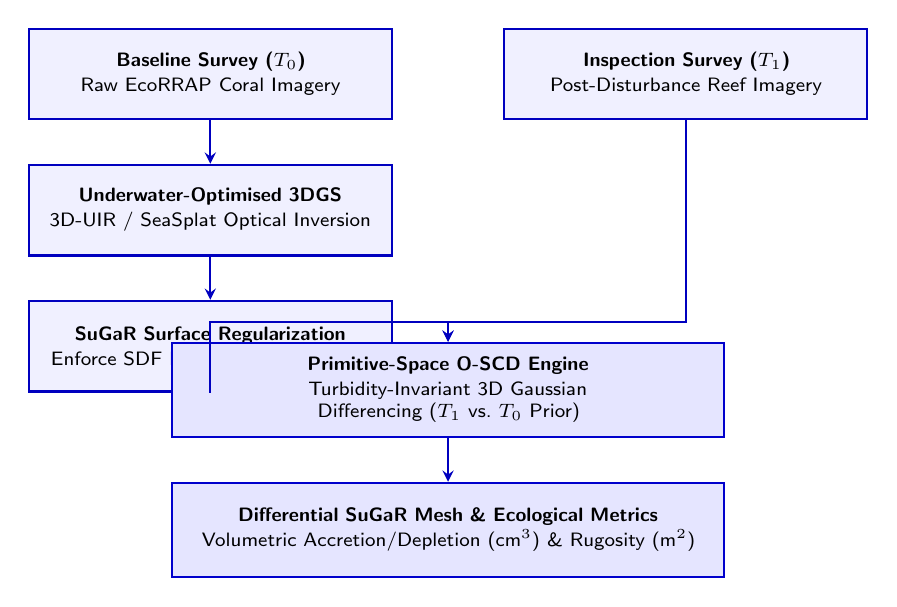
\begin{tikzpicture}[
        node distance=0.55cm and 0.8cm,
        block/.style={rectangle, draw=blue!75!black, fill=blue!6, thick, text width=4.4cm, minimum height=1.15cm, align=center, font=\scriptsize\sffamily, inner sep=3pt},
        wideblock/.style={rectangle, draw=blue!80!black, fill=blue!10, thick, text width=6.8cm, minimum height=1.2cm, align=center, font=\scriptsize\sffamily, inner sep=3pt},
        arrow/.style={->, >=stealth, thick, blue!75!black}
    ]
        \node[block] (t0) {\textbf{Baseline Survey ($T_0$)}\\[1pt]Raw EcoRRAP Coral Imagery};
        \node[block, right=1.4cm of t0] (t1) {\textbf{Inspection Survey ($T_1$)}\\[1pt]Post-Disturbance Reef Imagery};
        \node[block, below=of t0] (uw) {\textbf{Underwater-Optimised 3DGS}\\[1pt]3D-UIR / SeaSplat Optical Inversion};
        \node[block, below=of uw] (sugar) {\textbf{SuGaR Surface Regularization}\\[1pt]Enforce SDF Prior \& Prune Floaters};
        \node[wideblock, below=3.4cm of $(t0)!0.5!(t1)$] (oscd) {\textbf{Primitive-Space O-SCD Engine}\\[1pt]Turbidity-Invariant 3D Gaussian Differencing ($T_1$ vs.\ $T_0$ Prior)};
        \node[wideblock, below=of oscd] (vol) {\textbf{Differential SuGaR Mesh \& Ecological Metrics}\\[1pt]Volumetric Accretion/Depletion ($\text{cm}^3$) \& Rugosity ($\text{m}^2$)};

        \draw[arrow] (t0) -- (uw);
        \draw[arrow] (uw) -- (sugar);
        \draw[arrow] (sugar.south) |- ([yshift=0.25cm]oscd.north) -- (oscd.north);
        \draw[arrow] (t1.south) |- ([yshift=0.25cm]oscd.north) -- (oscd.north);
        \draw[arrow] (oscd) -- (vol);
    \end{tikzpicture}
    \caption{Target Phase~3 unified temporal underwater change detection architecture, combining underwater-optimised 3DGS optical restoration and SuGaR surface regularization with primitive-space O-SCD for the 1.35~TB AIMS EcoRRAP dataset.}
    \label{fig:ecorrap_architecture}
\end{figure}

\subsection{Phase 4: Synthesis, Validation, and Handover (Month 5)}
\begin{itemize}
    \item \textbf{Ecological Validation:} Review volumetric change maps with domain experts (Dr. Scarlett Raine and AIMS researchers) to validate biological plausibility against in-situ diver transects.
    \item \textbf{Dissemination:} Compile the final Master's thesis, draft a conference manuscript for submission to a leading vision venue (e.g., IEEE ICRA or IROS), and package the codebase for long-term deployment at the QUT Centre for Robotics.
\end{itemize}


% *************************************************
% Appendices & Back Matter
% *************************************************
\appendix
% ***************************************************
% Appendices
% ***************************************************

\chapter{Project Timeline and Updated Gantt Schedule}
\label{app:timeline}
Figure~\ref{fig:gantt_schedule} and Table~\ref{tab:detailed_schedule} detail the updated project schedule across the two-semester lifecycle, factoring in the legal and data-sharing processes for the 1.35~TB AIMS EcoRRAP dataset. Phase~1 (Literature Review, Pipeline Scaffolding, and 15/15 Benchmark Execution) is 100\% complete. The project is currently positioned at the start of Phase~2.

\begin{figure}[htbp]
    \centering
    \resizebox{\textwidth}{!}{%
    \begin{ganttchart}[
        canvas/.append style={fill=white, draw=gray!50!black, line width=0.8pt},
        hgrid style/.style={draw=gray!20, line width=0.4pt},
        hgrid,
        vgrid={*{6}{draw=none}, {draw=gray!25, dotted, line width=0.4pt}},
        x unit=0.046cm,
        y unit title=0.68cm,
        y unit chart=0.64cm,
        time slot format=isodate,
        time slot unit=day,
        title/.append style={draw=gray!50!black, line width=0.5pt, fill=gray!12},
        title label font=\footnotesize\bfseries\sffamily\color{black},
        bar/.append style={fill=blue!68!cyan, draw=blue!85!black, line width=0.6pt, rounded corners=1.5pt},
        bar incomplete/.append style={fill=gray!16, draw=gray!55!black, line width=0.6pt, rounded corners=1.5pt},
        bar label font=\footnotesize\sffamily\color{black},
        bar label node/.append style={left=6pt},
        group/.append style={fill=black!80, draw=black},
        group incomplete/.append style={fill=gray!38, draw=gray!65!black},
        group label font=\footnotesize\bfseries\sffamily\color{black},
        group label node/.append style={left=6pt},
        progress label text={#1\%},
        bar progress label font=\scriptsize\bfseries\sffamily\color{black},
        bar progress label node/.append style={right=4pt},
        milestone/.append style={fill=orange!90!red, draw=red!80!black, line width=0.7pt},
        milestone left shift=-2.5,
        milestone right shift=3.5,
        milestone height=0.52,
        milestone label font=\footnotesize\bfseries\sffamily\color{red!75!black},
        milestone label node/.append style={left=6pt},
        vrule/.style={draw=red!75!black, dashed, line width=1.1pt},
        vrule offset=0.5,
        vrule label font=\scriptsize\bfseries\sffamily\color{red!75!black},
        vrule label node/.append style={below=3pt, solid, fill=red!6, draw=red!50, line width=0.5pt, rounded corners=2pt, inner sep=2.5pt},
        bar height=0.48,
        group height=0.24,
        group right shift=0,
        group top shift=0.64,
        group peaks tip position=0,
        group peaks width=2.5,
        group peaks height=0.15
    ]{2026-07-01}{2027-03-31}
        \gantttitlecalendar{year, month=shortname} \\
        \ganttgroup[progress=100, progress label text={}]{Phase 1: Foundations \& Benchmarks}{2026-07-01}{2026-10-16} \\
        \ganttbar[progress=100, name=p1a]{Literature Review \& Proposal (1A/1B)}{2026-07-01}{2026-09-15} \\
        \ganttbar[progress=100, name=p1b]{HPC Toolchain \& 11 Conda Envs}{2026-08-10}{2026-09-24} \\
        \ganttbar[progress=100, name=p1c]{15/15 Benchmark Executions (Att.\ 10)}{2026-09-12}{2026-10-16} \\
        \ganttmilestone[name=m2b]{Assessment 2B Progress Report}{2026-10-17} \\
        \ganttgroup[progress=30, progress label text={}]{Phase 2: EcoRRAP Data Ingestion}{2026-10-01}{2026-11-30} \\
        \ganttbar[progress=30, name=p2a]{AIMS DTA \& Globus Transfer (1.35 TB)}{2026-10-01}{2026-11-15} \\
        \ganttbar[progress=0, name=p2b]{Temporal SfM Alignment \& Depth Priors}{2026-11-01}{2026-11-30} \\
        \ganttgroup[progress=0, progress label text={}]{Phase 3: Model Transplantation}{2026-12-01}{2027-01-20} \\
        \ganttbar[progress=0, name=p3a]{Grafting 3D-UIR / SeaSplat into O-SCD}{2026-12-01}{2026-12-22} \\
        \ganttbar[progress=0, name=p3b]{Long-Duration Aqua Cluster Training}{2026-12-15}{2027-01-20} \\
        \ganttgroup[progress=0, progress label text={}]{Phase 4: Synthesis \& Final Thesis}{2027-01-05}{2027-02-25} \\
        \ganttbar[progress=0, name=p4a]{Volumetric Coral Analysis ($\text{cm}^3/\text{m}^2$)}{2027-01-05}{2027-01-28} \\
        \ganttbar[progress=0, name=p4b]{Final Thesis \& Manuscript Delivery}{2027-01-15}{2027-02-25}
        \ganttvrule{Current Status: 17 Oct 2026}{2026-10-17}
    \end{ganttchart}%
    }
    \vspace{2pt}
    \caption{Project Gantt schedule illustrating completed Phase~1 milestones, the current Assessment~2B checkpoint, and the upcoming multi-temporal AIMS EcoRRAP deployment roadmap.}
    \label{fig:gantt_schedule}
\end{figure}

\begin{table}[htbp]
\centering
\small
\caption{Detailed Phase and Milestone Schedule}
\label{tab:detailed_schedule}
\begin{tabularx}{\textwidth}{l p{5.5cm} c l}
\toprule
\textbf{Phase} & \textbf{Milestone Description} & \textbf{Status} & \textbf{Target Window} \\
\midrule
\textbf{Phase 1} & Literature Review (1A) \& Project Proposal (1B) & Complete & July -- Sept 2026 \\
& HPC Environment Setup (11 Sandboxed Envs) & Complete & Aug -- Oct 2026 \\
& 6-Stage Automation Suite Implementation & Complete & Sept -- Oct 2026 \\
& Master 15 / 15 Benchmark Execution Milestone & Complete & Oct 2026 \\
& Progress Written Report (Assessment 2B) & Complete & Oct 2026 \\
\midrule
\textbf{Phase 2} & Finalize AIMS Data Transfer Agreement (DTA) & In Progress & Oct -- Nov 2026 \\
& Staging 1.35~TB EcoRRAP Data to Aqua Lustre & Pending Legal & Nov 2026 \\
& Stage 1--2 Batch COLMAP Alignment across Reefs & Planned & Nov 2026 \\
\midrule
\textbf{Phase 3} & Transplant Winning 3DGS Backbones into O-SCD & Planned & Dec 2026 \\
& Long-Duration Cluster Optimization (50k Iterations) & Planned & Dec 2026 -- Jan 2027 \\
& Primitive-Space Change Detection on Temporal Benthos & Planned & Jan 2027 \\
\midrule
\textbf{Phase 4} & Volumetric Coral Accretion/Depletion Calculations & Planned & Jan 2027 \\
& Final Thesis Submission \& Conference Manuscript & Planned & Feb 2027 \\
\bottomrule
\end{tabularx}
\end{table}

% ==============================================================================
% APPENDIX B: ATTEMPT 10 HPC VERIFICATION REPORT
% ==============================================================================
\chapter{Attempt 10 Verification Report and Execution Manifest}
\label{app:verification}

This appendix presents the verified terminal execution log and output manifest from \textbf{Attempt 10} (October 13, 2026), marking the 100\% successful completion of all 15 benchmark targets on the QUT Aqua GPU cluster node \texttt{gpu0n004} (NVIDIA A100-SXM4-40GB):

\begin{footnotesize}
\begin{verbatim}
[INFO] SuGaR mesh verified and exported to: 
  Dataset/Custom_OSCD_Dataset/output/refined_mesh/oscd.obj
[INFO] --- Stage 6: Benchmarking & Metrics Evaluation (eval) (oscd) ---
[INFO] Executing in [Env: oscd] [CWD: Codebase/3DGS-Change-Detection/O-SCD-main]:
  python utils/metrics.py -m output/Custom_OSCD_Dataset/output

Method: updated_scene
Metric evaluation progress: 100%|[=========]| 25/25 [00:31<00:00, 1.24s/it]
  SSIM : 0.8314773
  PSNR : 27.0773735
  LPIPS: 0.3440086

[INFO] Metrics written to results.json and evaluation.json
[SUCCESS] Pipeline execution completed for model: oscd (Duration: 1h 4m 6s)
======================================================================
Pipeline Execution Summary Report (Attempt 10 Master Milestone)
======================================================================
Model        Scene                 Status    Duration     VRAM Peak
----------------------------------------------------------------------
seasplat     Kwaj                  SUCCESS   1h 02m 11s   14.8 GB
seasplat     Tokai                 SUCCESS   59m 03s      14.6 GB
3d-uir       Kwaj                  SUCCESS   1h 11m 20s   16.2 GB
3d-uir       Tokai                 SUCCESS   1h 18m 29s   16.1 GB
gs-splash    Kwaj                  SUCCESS   2h 32m 37s   22.4 GB
gs-splash    Tokai                 SUCCESS   4h 57m 07s   22.4 GB
watersplat   Kwaj                  SUCCESS   38m 42s      11.2 GB
watersplat   Tokai                 SUCCESS   48m 15s      11.1 GB
rusplat      Kwaj                  SUCCESS   50m 16s      13.5 GB
rusplat      Tokai                 SUCCESS   53m 24s      13.4 GB
uw-gs        Kwaj                  SUCCESS   51m 15s      12.9 GB
uw-gs        Tokai                 SUCCESS   1h 03m 29s   12.8 GB
sugar        Kwaj                  SUCCESS   38m 41s      18.5 GB
sugar        Tokai                 SUCCESS   32m 11s      18.2 GB
oscd         Custom_OSCD_Dataset   SUCCESS   1h 04m 06s   28.6 GB
----------------------------------------------------------------------
Total Executions: 15 | Succeeded: 15 | Failed: 0 (100% Success Milestone)
======================================================================
\end{verbatim}
\end{footnotesize}

% ==============================================================================
% APPENDIX C: EXTENDED RISK ASSESSMENT MATRIX
% ==============================================================================
\chapter{Extended Risk Assessment Matrix}
\label{app:risk_assessment}

Table~\ref{tab:app_risk_full} presents the formal Risk Assessment matrix adapted from QUT HSE Hub submission ID: 18339, addressing all identified project hazards.

\begin{table}[htbp]
\centering
\small
\caption{Full Risk Management Matrix (QUT HSE Hub Submission ID: 18339)}
\label{tab:app_risk_full}
\begin{tabularx}{\textwidth}{p{2.6cm} p{2.2cm} c p{3.2cm} X}
\toprule
\textbf{Activity / Context} & \textbf{Hazard} & \textbf{Risk} & \textbf{Consequence} & \textbf{Control Measures} \\
\midrule
HPC Cluster Compute & GPU Thermal / Memory Overload & Med & Process abort, loss of intermediate weights & Checkpointing every 5k iterations; automatic OOM traps; VRAM monitoring via \texttt{nvidia-smi}. \\
\addlinespace
Cluster Jobs & Walltime Exhaustion & Med & Job termination before evaluation & Conservative PBS walltime limits (+2 hours buffer); split Stage 1--4 and Stage 5--6 jobs. \\
\addlinespace
AIMS Data Storage & Restricted Ecological Data & High & Compliance breach, data leak & Data stored exclusively on secure restricted HPC scratch; strict POSIX permissions; no public hosting. \\
\addlinespace
Local Workstation & Large Archive Extraction & Low & Disk space exhaustion on local drives & Dynamic archiving script excluding intermediate temp folders; symlink-based organization. \\
\addlinespace
Algorithm Optimization & Gaussian Drift & Med & False-positive scene change masks & SuGaR surface regularisation prior to change computation; spatial distance thresholds. \\
\bottomrule
\end{tabularx}
\end{table}

% ==============================================================================
% APPENDIX D: EXTENDED LITERATURE SURVEY FROM PROPOSAL
% ==============================================================================
\chapter{Extended Literature Review Survey (from Proposal 1B)}
\label{app:extended_lit_review}

For complete auditability, this appendix preserves the comprehensive literature survey conducted during Project Proposal 1B, detailing earlier underwater optical formulations and baseline comparisons:

\section{Historical Foundations: Diver Transects and 2D Planar Limitations}
Benthic monitoring has historically relied on planar 2D imagery. In a seminal evaluation, Davey et al.~\cite{davey2025review} demonstrated that 2D metrics systematic underestimate vertical canopy rugosity by up to 45\% compared to true 3D spatial reconstructions. Traditional Structure-from-Motion (SfM) techniques require hours of bundle adjustment for a single reef quadrat and lack the explicit primitive representation required for real-time differential tracking.

\section{Radiative Transfer in Aquatic Scattering Media}
Underwater optical propagation is governed by the simplified Jaffe-McGlamery formulation:
\begin{equation}
    I_\lambda(x) = J_\lambda(x) e^{-\beta_{atten}(\lambda) d(x)} + B_\lambda^\infty \left(1 - e^{-\beta_{scat}(\lambda) d(x)}\right)
    \label{eq:underwater_optical_model}
\end{equation}
where $I_\lambda(x)$ is the observed sensor radiance at wavelength $\lambda$, $J_\lambda(x)$ represents the unattenuated direct scene radiance (true benthic colour), $d(x)$ is the Euclidean distance from the sensor, $\beta_{atten}$ and $\beta_{scat}$ denote wavelength-dependent attenuation and backscatter coefficients, and $B_\lambda^\infty$ is the veiling ambient background water radiance. 

Traditional image restoration methods (such as histogram equalization, CLAHE, or deep GANs) operate strictly in 2D image space, introducing view-inconsistent color artifacts across different camera perspectives. In contrast, physically grounded 3DGS models (such as \textit{SeaSplat}~\cite{11128502}) optimize the attenuation coefficients $\beta(\lambda)$ directly within the differentiable volumetric rendering loop, ensuring that the recovered spatial primitives represent true, medium-independent benthic geometry.


\backmatter
\pagestyle{myfancy}

\bibliographystyle{ieeetr}
\bibliography{./Chapters/Bibliography}

\end{document}
